%%% The main file. It contains definitions of basic parameters and includes all other parts.

% Meta-data of your thesis (please edit)
\input metadata.tex

% Generate metadata in XMP format for use by the pdfx package
\input xmp.tex

%% Settings for single-side (simplex) printing
% Margins: left 40mm, right 25mm, top and bottom 25mm
% (but beware, LaTeX adds 1in implicitly)
\documentclass[12pt,a4paper]{report}
\setlength\textwidth{145mm}
\setlength\textheight{247mm}
\setlength\oddsidemargin{15mm}
\setlength\evensidemargin{15mm}
\setlength\topmargin{0mm}
\setlength\headsep{0mm}
\setlength\headheight{0mm}
% \openright makes the following text appear on a right-hand page
\let\openright=\clearpage

%% Settings for two-sided (duplex) printing
% \documentclass[12pt,a4paper,twoside,openright]{report}
% \setlength\textwidth{145mm}
% \setlength\textheight{247mm}
% \setlength\oddsidemargin{14.2mm}
% \setlength\evensidemargin{0mm}
% \setlength\topmargin{0mm}
% \setlength\headsep{0mm}
% \setlength\headheight{0mm}
% \let\openright=\cleardoublepage

%% If the thesis has no printed version, symmetric margins look better
% \documentclass[12pt,a4paper]{report}
% \setlength\textwidth{145mm}
% \setlength\textheight{247mm}
% \setlength\oddsidemargin{10mm}
% \setlength\evensidemargin{10mm}
% \setlength\topmargin{0mm}
% \setlength\headsep{0mm}
% \setlength\headheight{0mm}
% \let\openright=\clearpage

%% Generate PDF/A-2u
\usepackage[a-2u]{pdfx}

%% Prefer Latin Modern fonts
\usepackage{lmodern}
% If we are not using LuaTeX, we need to set up character encoding:
\usepackage{iftex}
\ifpdftex
\usepackage[utf8]{inputenc}
\usepackage[T1]{fontenc}
\usepackage{textcomp}
\fi

%% Further useful packages (included in most LaTeX distributions)
\usepackage{amsmath}        % extensions for typesetting of math
\usepackage{amsfonts}       % math fonts
\usepackage{amsthm}         % theorems, definitions, etc.
\usepackage{bm}             % boldface symbols (\bm)
\usepackage{booktabs}       % improved horizontal lines in tables
\usepackage{caption}        % custom captions of floating objects
\usepackage{dcolumn}        % improved alignment of table columns
\usepackage{floatrow}       % custom float environments
\usepackage{graphicx}       % embedding of pictures
\usepackage{indentfirst}    % indent the first paragraph of a chapter
\usepackage[nopatch=item]{microtype}   % micro-typographic refinement
\usepackage{paralist}       % improved enumerate and itemize
\usepackage[nottoc]{tocbibind} % makes sure that bibliography and the lists
			    % of figures/tables are included in the table
			    % of contents
\usepackage{xcolor}         % typesetting in color

% The hyperref package for clickable links in PDF and also for storing
% metadata to PDF (including the table of contents).
% Most settings are pre-set by the pdfx package.
\hypersetup{unicode}
\hypersetup{breaklinks=true}

% Packages for computer science theses
\usepackage{algpseudocode}  % part of algorithmicx package
\usepackage{algorithm}
\usepackage{fancyvrb}       % improved verbatim environment
\usepackage{listings}       % pretty-printer of source code

% MY PACKAGES
\usepackage{csquotes}

% You might want to use cleveref for references
% \usepackage{cleveref}

% Set up formatting of bibliography (references to literature)
% Details can be adjusted in macros.tex.
%
% BEWARE: Different fields of research and different university departments
% have their own customs regarding bibliography. Consult the bibliography
% format with your supervisor.
%
% The basic format according to the ISO 690 standard with numbered references
\usepackage[natbib,style=iso-numeric,sorting=none]{biblatex}
% ISO 690 with alphanumeric references (abbreviations of authors' names)
%\usepackage[natbib,style=iso-alphabetic]{biblatex}
% ISO 690 with references Author (year)
%\usepackage[natbib,style=iso-authoryear]{biblatex}
%
% Some fields of research prefer a simple format with numbered references
% (sorting=none tells that bibliography should be listed in citation order)
%\usepackage[natbib,style=numeric,sorting=none]{biblatex}
% Numbered references, but [1,2,3,4,5] is compressed to [1-5]
%\usepackage[natbib,style=numeric-comp,sorting=none]{biblatex}
% A simple format with alphanumeric references:
%\usepackage[natbib,style=alphabetic]{biblatex}

% Load the file with bibliography entries
\addbibresource{bibliography.bib}

% Our definitions of macros (see description inside)
\input macros.tex

%%% Title page and various mandatory informational pages
\begin{document}
%%% Title page of the thesis and other mandatory pages

%%% Title page of the thesis

\pagestyle{empty}
\hypersetup{pageanchor=false}
\begin{center}

\centerline{\mbox{
\includegraphics[width=166mm]{../img/logo-en.pdf}}}

\vspace{-8mm}
\vfill

{\bf\Large BACHELOR THESIS}

\vfill

{\LARGE\ThesisAuthor}

\vspace{15mm}

{\LARGE\bfseries\ThesisTitle}

\vfill

\Department

\vfill

{
\centerline{\vbox{\halign{\hbox to 0.45\hsize{\hfil #}&\hskip 0.5em\parbox[t]{0.45\hsize}{\raggedright #}\cr
Supervisor of the bachelor thesis:&\Supervisor \cr
\noalign{\vspace{2mm}}
Study programme:&\StudyProgramme \cr
\noalign{\vspace{2mm}}
Study branch:&\StudyBranch \cr
}}}}

\vfill

% Zde doplňte rok
Prague \YearSubmitted

\end{center}

\newpage

%%% Here should be a bound sheet included -- a signed copy of the "bachelor
%%% thesis assignment". This assignment is NOT a part of the electronic
%%% version of the thesis. DO NOT SCAN.

%%% A page with a solemn declaration to the bachelor thesis

\openright
\hypersetup{pageanchor=true}
\pagestyle{plain}
\pagenumbering{roman}
\vglue 0pt plus 1fill

\noindent
I declare that I carried out this bachelor thesis independently, and only with the cited
sources, literature and other professional sources. It has not been used to obtain another
or the same degree.

\medskip\noindent
I understand that my work relates to the rights and obligations under the Act No.~121/2000 Sb.,
the Copyright Act, as amended, in particular the fact that the Charles
University has the right to conclude a license agreement on the use of this
work as a school work pursuant to Section 60 subsection 1 of the Copyright~Act.

\vspace{10mm}

\hbox{\hbox to 0.5\hsize{%
In \hbox to 6em{\dotfill} date \hbox to 6em{\dotfill}
\hss}\hbox to 0.5\hsize{\dotfill\quad}}
\smallskip
\hbox{\hbox to 0.5\hsize{}\hbox to 0.5\hsize{\hfil Author's signature\hfil}}

\vspace{20mm}
\newpage

%%% Dedication

\openright

\noindent
\Dedication

\newpage

%%% Mandatory information page of the thesis

\openright

\vbox to 0.5\vsize{
\setlength\parindent{0mm}
\setlength\parskip{5mm}

Title:
\ThesisTitle

Author:
\ThesisAuthor

\DeptType:
\Department

Supervisor:
\Supervisor, \SupervisorsDepartment

Abstract:
\Abstract

Keywords:
\Keywords

\vss}

\newpage

\openright
\pagestyle{plain}
\pagenumbering{arabic}
\setcounter{page}{1}


%%% A page with automatically generated table of contents of the thesis

\tableofcontents

%%% Each chapter is kept in a separate file
\chapter{Introduction}

\todo{Games exist. They are good. I like games. I will make a game.}

\section{Game Genre}

There are a plethora of games. Each is unique in its own way, but there are many similarities among them. One of the ways to categorize games is by their genre. A genre can encompass many characteristics of a game, most often its mechanics, but also its theme, art style or the medium it is played on. Genres have no exact definitions or strict boundaries and similarly, any individual game is usually a mix of different genres.

\subsection{Strategy}

One major genre is strategy games. Strategy games focus on tactics and long term planning. They require a lot of thinking. There are various kinds of strategy games, but most often, players compete against each other to reach some goal. These players can be real humans or artificial intelligence agents. Strategy games often utilize hidden information or rely on the unpredictability of other players' actions to create an environment where there is no single best way to reach the goal. This means that players have to have a good understanding of the game and be able to adapt to the situation at hand.

There are many qualities players enjoy in strategy games. Of course, it feels great to outsmart your opponent or conquer a challenge. But strategy games also provide a sense of progression and accomplishment because of their depth. They are often very replayable because of the different situations that can arise from the game's mechanics.

One way to categorize a strategy game is whether is it real-time or turn-based. In turn-based strategy, players take turns to make their moves. This allows for a slower pace and more time to think about the best move. In real-time strategy games, however, the environment evolves continuously and players have to react and make decisions quickly.

\subsection{Tower Defense}

Tower defense is a subgenre of real-time strategy where the player has to defend against waves of enemies. The player has to build towers, which attack the enemies as they approach, in order to defend their base. The attackers are very predictable and usually follow a set path. The player has to build their towers in a way that maximizes their effectiveness against the attackers.
\?{do I want images and examples}

The game usually consist of multiple levels, each presenting a different challenge. The player has to adapt to the different attackers and the different terrain. Sometimes the levels make up a campaign, where the player has to progress through harder and harder levels to reach the end. Other times, the levels are standalone and the player can choose which level to play, where the goal can be to survive as long as possible. This can take a few hours and may become very repetitive.

The attackers can have unique abilities or be resistant to certain types of towers. The composition of each wave can be predetermined or randomized to a varying degree. In this way, the game can force the player to adapt and use different strategies. To make their decisions interesting, the player has various towers and upgrades at their disposal, each with different abilities, often complimenting each other.

Players can get resources to build their defense passively, but some tower defense games also include an economy system. Here, the player has to build economic buildings to generate the resources. This adds another layer of strategy to the game, as the player has to balance their economy with their defense.

\subsection{Rogue-like}

Rogue-like is a subgenre of role-playing games. In role-playing games, the player takes on the role of a character and goes on an adventure. The character can grow stronger by acquiring new abilities, items or experience. The player has to make decisions about how to upgrade their characters in order to overcome the challenges they might face. This high level of customization and the sense of progression makes role-playing games very engaging.

Rogue-like is named after the game Rogue, released in 1980\?{citation!}. The game was known for its high difficulty and the fact that the player had to start from the beginning if they died. The game is usually procedurally generated, meaning that the levels are created by an algorithm, rather than being designed by a human. This is important, because the player can't memorize the levels and has to rely on their skill and knowledge of the game's mechanics to progress. Since all in-game progress is lost when the player dies, the player has to learn from their mistakes and improve their skill in order to advance further. These are defining characteristics of rogue-likes which separate them from other role-playing games.

In most rogue-like games, you explore a dungeon, where you have to fight enemies and avoid traps. You are then rewarded with items and other resources to improve your character. The game is usually turn-based, making it more strategic.

There are many games which break the traditional rogue-like formula, but still share many of its characteristics. They might have a different theme, where you don't even fight monsters but instead compete in another task. They might include a progression system, where you unlock new items or upgrades for your future runs. Real-time gameplay is also common, where more skills are tested than just the player's ability to think strategically. These games are often called rogue-lites, however, we will not make such a distinction since all genres can be bent and blended in many ways. \?{do I include more examples here}

\subsection{Combining the two}

I enjoy playing both rogue-likes and tower defense games a lot\?{should this be here}. There aren't many games which combine these two genres. It is possible that this combination doesn't work well, however, it is worth exploring, because these two genres seem to compliment each other. This is why this game will be a blend of these two genres.

The main gameplay loop will be a tower defense game. The player will play through many short levels. Tower defense can get a bit stale, if you find a strategy that just works and you can use it every time. This is how some rogue-like elements can help. Each level will be procedurally generated featuring different terrain and attackers. Additionally, the player will start with a small arsenal of towers and other blueprints, and acquire new ones from a randomized selection as they progress. This means that the player will likely use a different strategy in each run.

\section{Original vision}

- player hops from planet to planet with their spaceship, stopping to refuel on each one. Here they have to defend until they get enough fuel to move on

- build economic buildings, build towers, defend against waves - balance economy, defense and offense

- each planet will have different terrain and attackers

- slowly, they will acquire new blueprints for defensive towers, economic buildings and other upgrades. These will be randomized, so you can't rely on the same strategy every time

- along the way, there will be events, shops, harder battles and other anomalies that the player can choose to interact with

- there will be some sort of story motivating why the player is going on this perilous journey

\section{Current scope}

- a prototype

- playable battles - we can start play testing the core gameplay

- all necessary battle systems to add more content later

- progressing through levels and collecting blueprints to test which blueprints work well (provide new strategies, are balanced)

\subsection{Goals}

\chapter{Game Design}

Before we start implementing the game, we should design its individual parts.
We need to decide which mechanics will be in the game and how will the player interact with them.
The game needs to react to the player's actions and communicate the information the player should know.
This all depends on what exactly are we trying to achieve.
Thus, we should set some design goals.

\section{Design goals}

We aim to make the game's mechanics clear, and controls intuitive and responsive.
This is a necessity for every game because without this, the players can't even properly play the game you want them to play.
We won't make a subsection specifically for this goal, but it will inform many of our decisions throughout the design.

The following are the goals specific for our game.
We will look at other games for inspiration how these goals could be reached.
The prototype won't achieve any of them well, but they still inform the design of the mechanics we will implement.

\begin{enumerate}
    \item \nameref{sec:goal-depth-battle}
    \item \nameref{sec:goal-depth-run}
    \item \nameref{sec:goal-various-builds}
    \item \nameref{sec:goal-force-exploration}
    \item \nameref{sec:goal-challenge}
\end{enumerate}

\subsection{Strategic Depth in Every Battle} \label{sec:goal-depth-battle}

The player should make meaningful strategic decisions throughout every battle.
Each battle should be different enough to require the player to adapt to the current situation.
This is where the action will happen, but we want the player to make tactical decisions, not test their reflexes.
With this constraint, battles would be boring if every one played out the same.

In \emph{Plants vs.\ Zombies}, the player wants to plant \emph{Sunflowers} or other \emph{sun}-producing plants.
The more they build their economy, the more plants they can afford in the future.
However, these plants can't kill zombies, so the goal is to spend the bare minimum on defense.
This is a hard problem to solve, since when and where zombies will appear is not completely predictable.
What makes this even more complicated are cheap single-use plants like the \emph{Potato Mine}.
It costs only 25\,\emph{sun} and can kill almost any zombie, where, for example, a \emph{Peashooter} costs 100\,\emph{sun}, but is permanent and able to kill tens of zombies over the course of a level.
This means the player always has to consider if it's better to place a plant that's the best now or a plant that will be the best in the future.

\begin{center}
    \captionsetup{type=figure}
    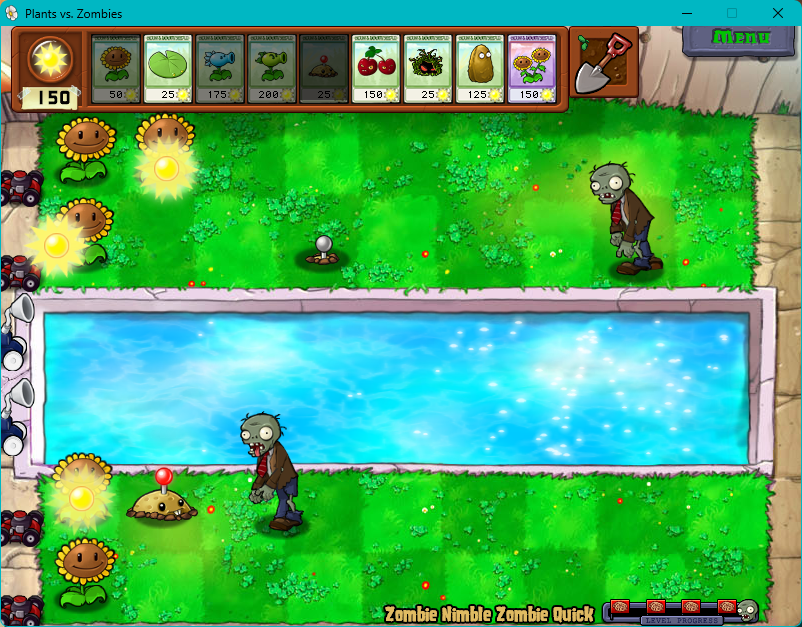
\includegraphics[width=0.8\textwidth]{img/Plants-vs-Zombies-Mines.png}
    \caption{\emph{Sunflowers} and \emph{Potato Mines} in \emph{Plants vs.\ Zombies}. \emph{Sunflowers} are necessary to fuel your economy, while \emph{Potato Mines} are a cheap way to deal with the first few zombies.}
    \label{fig:pvz-mines}
\end{center}

In \emph{Slay the Spire}, the player has to make a similar kind of decision, but even more often.
Almost every enemy grows stronger over time, or makes the player character weaker as they fight.
This means that the player always has to consider when it's the best to defend and when it's better to attack.
The player can choose to not block some damage now in order to kill the enemy sooner and prevent bigger attacks in the future.
The player also has to plan several turns in advance because many cards have longer lasting effects.
\enquote{Is it better to play a card that makes me stronger in the future or a card that helps me now?}

Every fight is different because every enemy has distinctive behavior.
Some enemies get much more powerful over time, so it is important to kill them quickly.
Others punish the player for attacking them, so the player needs to kill them with precision.
Fights also vary a lot because the player draws their cards in a different order every time.
All this means that the player has something to think about every turn.

Our game will also have economic buildings and instant abilities, so the player has to balance economy and short-term versus long-term defense.
The player will have to survive some number of waves, but they will be able to spend extra materials to mine fuel faster and end the battle sooner.
This is similar to being more offensive in \emph{Slay the Spire}, since the waves of attackers should get stronger at a faster pace than the player's defense.
Each battle will require a different approach, since the waves will be composed of a different set of attackers every time.
We can also vary the nature of a battle by changing up the terrain and making attacker paths different lengths or more numerous.
This might seem like too much, but we want to playtest all these options and possibly cut those, which don't work well.

\subsection{Strategic Depth in Every Run} \label{sec:goal-depth-run}

The player should make meaningful strategic decisions throughout every run and there should be no clear path to victory.

In \emph{Slay the Spire}, the player needs to improve many aspects of their deck in tandem.
They need to have great defensive cards, cards that can deal with enemies that have a lot of health, cards that can attack multiple enemies at once and more.
The player should also care about the average cost of the cards in their deck.
It is bad when the player wants to both defend and attack on a given turn, but they've drawn only an expensive attack and an expensive defensive card.
It is also suboptimal when the player plays out all the cards they've drawn, but they have leftover energy they didn't spend.
Balancing these aspects of the deck leads to some difficult decisions when picking cards to add.
For example, should the player pick a good defensive card because they are lacking in defense, or should they pick an attack that's just very strong.

We want to balance the battles in a way, which requires the player to have strong blueprints with various qualities.
The players should need good economic buildings, fuel-producing buildings, abilities and towers good at dealing with various kinds of attackers.
They should also have some cheaper towers to build in the first few waves and more expensive towers to build once they produce a lot of material.

In \emph{Slay the Spire}, the player come across an interesting trade-off between short-term and long-term power, even in building their deck.
The player wants cards which will have a great potential to be strong in the future, having great synergy with other cards.
But these cards aren't strong right now and the player needs to survive the next few fights, making them choose cards that are useful immediately, but might not be as powerful later in the run.
As an example we can look at \emph{Iron Wave} and \emph{Double Tap}.

\begin{center}
    \captionsetup{type=figure}
    \begin{minipage}{.25\textwidth}
        \centering
        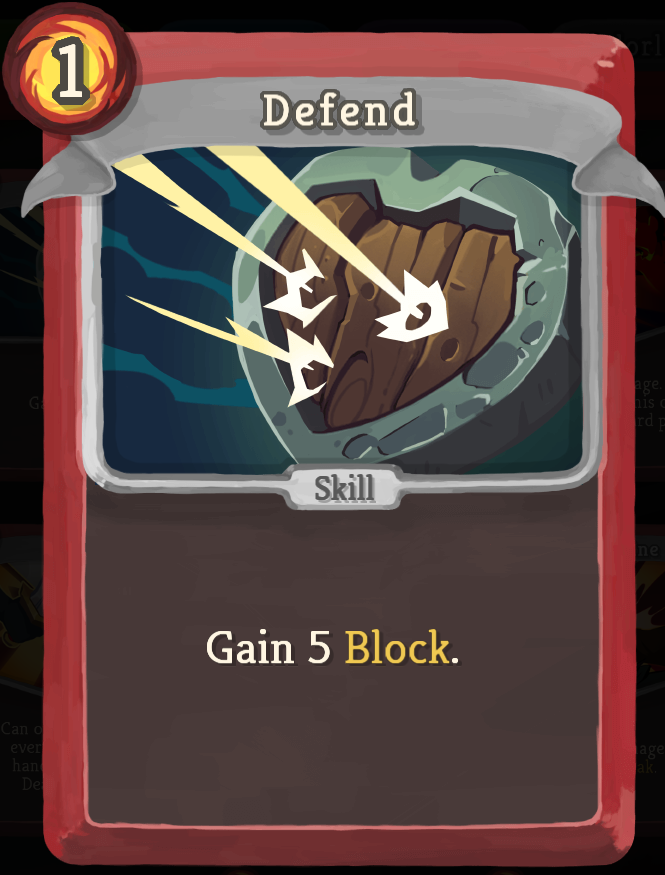
\includegraphics[width=0.95\textwidth]{img/Slay-the-Spire-Defend.png}
        \label{fig:sts-defend}
    \end{minipage}%
    \begin{minipage}{.25\textwidth}
        \centering
        \captionsetup{justification=centering}
        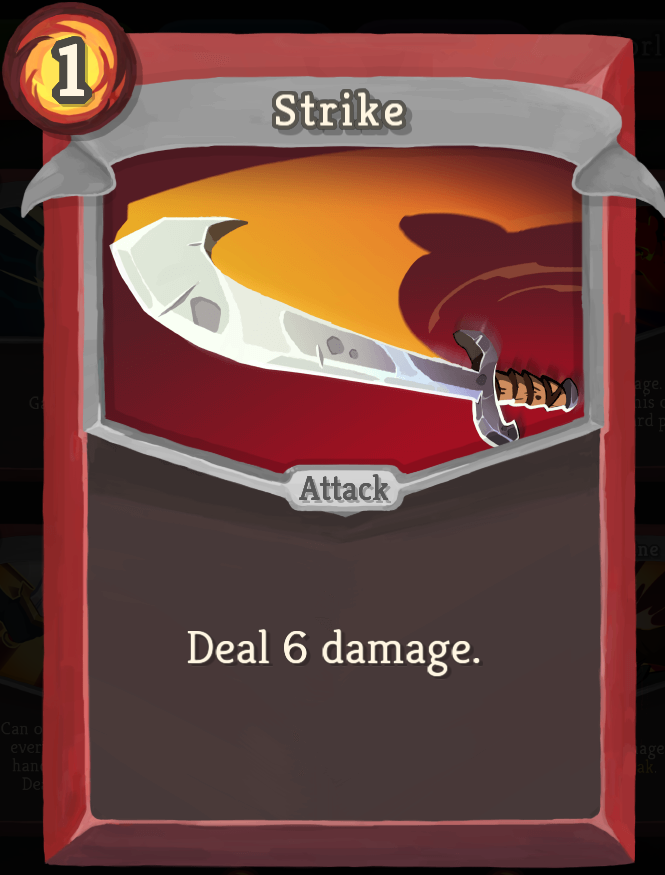
\includegraphics[width=0.95\textwidth]{img/Slay-the-Spire-Strike.png}
        \label{fig:sts-strike}
    \end{minipage}%
    \begin{minipage}{.25\textwidth}
        \centering
        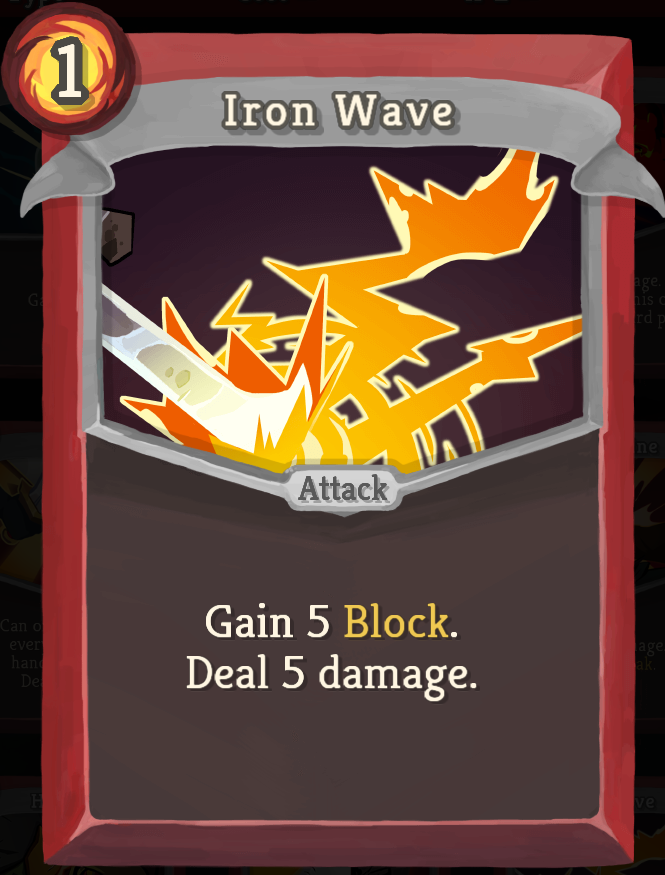
\includegraphics[width=0.95\textwidth]{img/Slay-the-Spire-Iron-Wave.png}
        \label{fig:sts-iron-wave}
    \end{minipage}%
    \begin{minipage}{.25\textwidth}
        \centering
        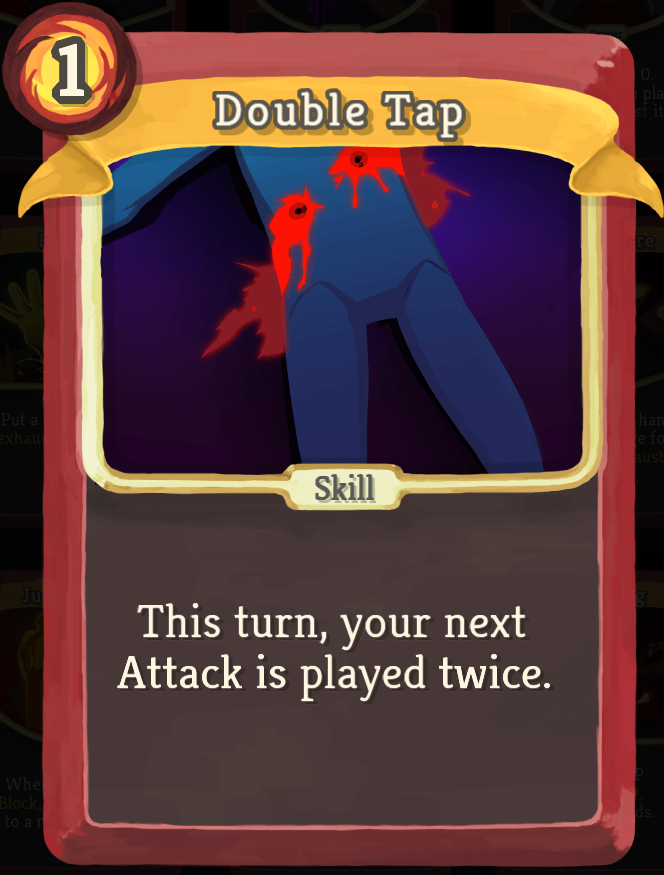
\includegraphics[width=0.95\textwidth]{img/Slay-the-Spire-Double-Tap.png}
        \label{fig:sts-double-tap}
    \end{minipage}
    \caption{\emph{Defend}, \emph{Strike}, \emph{Iron Wave} and \emph{Double Tap}---cards from \emph{Slay the Spire.}}
\end{center}

\?{Should I transcribe the cards}
The player starts each run with several copies of \emph{Defend} and \emph{Strike} in their deck.
Compared to them, \emph{Iron Wave} is very cost-efficient.
It does almost the same thing as \emph{Defend} \textbf{and} \emph{Strike} combined, but for the cost of 1\,\emph{energy}, the same as \emph{Defend} \textbf{or} \emph{Strike}.
Picking this card can help a lot in the early fights, however, it doesn't really grow stronger later in the run.
\emph{Double Tap}, on the other hand, is not great at the start.
In essence, it acts like another \emph{Strike} most of the time, and is useful only when the player draws another attack alongside it.
It is however very strong when your deck contains many attacks that cost a lot of energy but deal much more damage.
Then it allows the player to play a powerful attack twice at the cost of only one more energy.
We can design the blueprints in our game similarly, making some useful early in the run and some powerful later.

\subsection{Make Various Builds Viable} \label{sec:goal-various-builds}

The player should be able to beat the game with a lot of different combinations of blueprints.
We want the player to experiment with different builds, but that will never happen if only few of them are good enough.

- StS --- some cards interact in interesting ways that make them stronger ; there are cards and relics which fundamentally change the way your deck works (ex. barricade and entrench) nerfing some builds is important

\begin{figure}[htb]
    \centering
    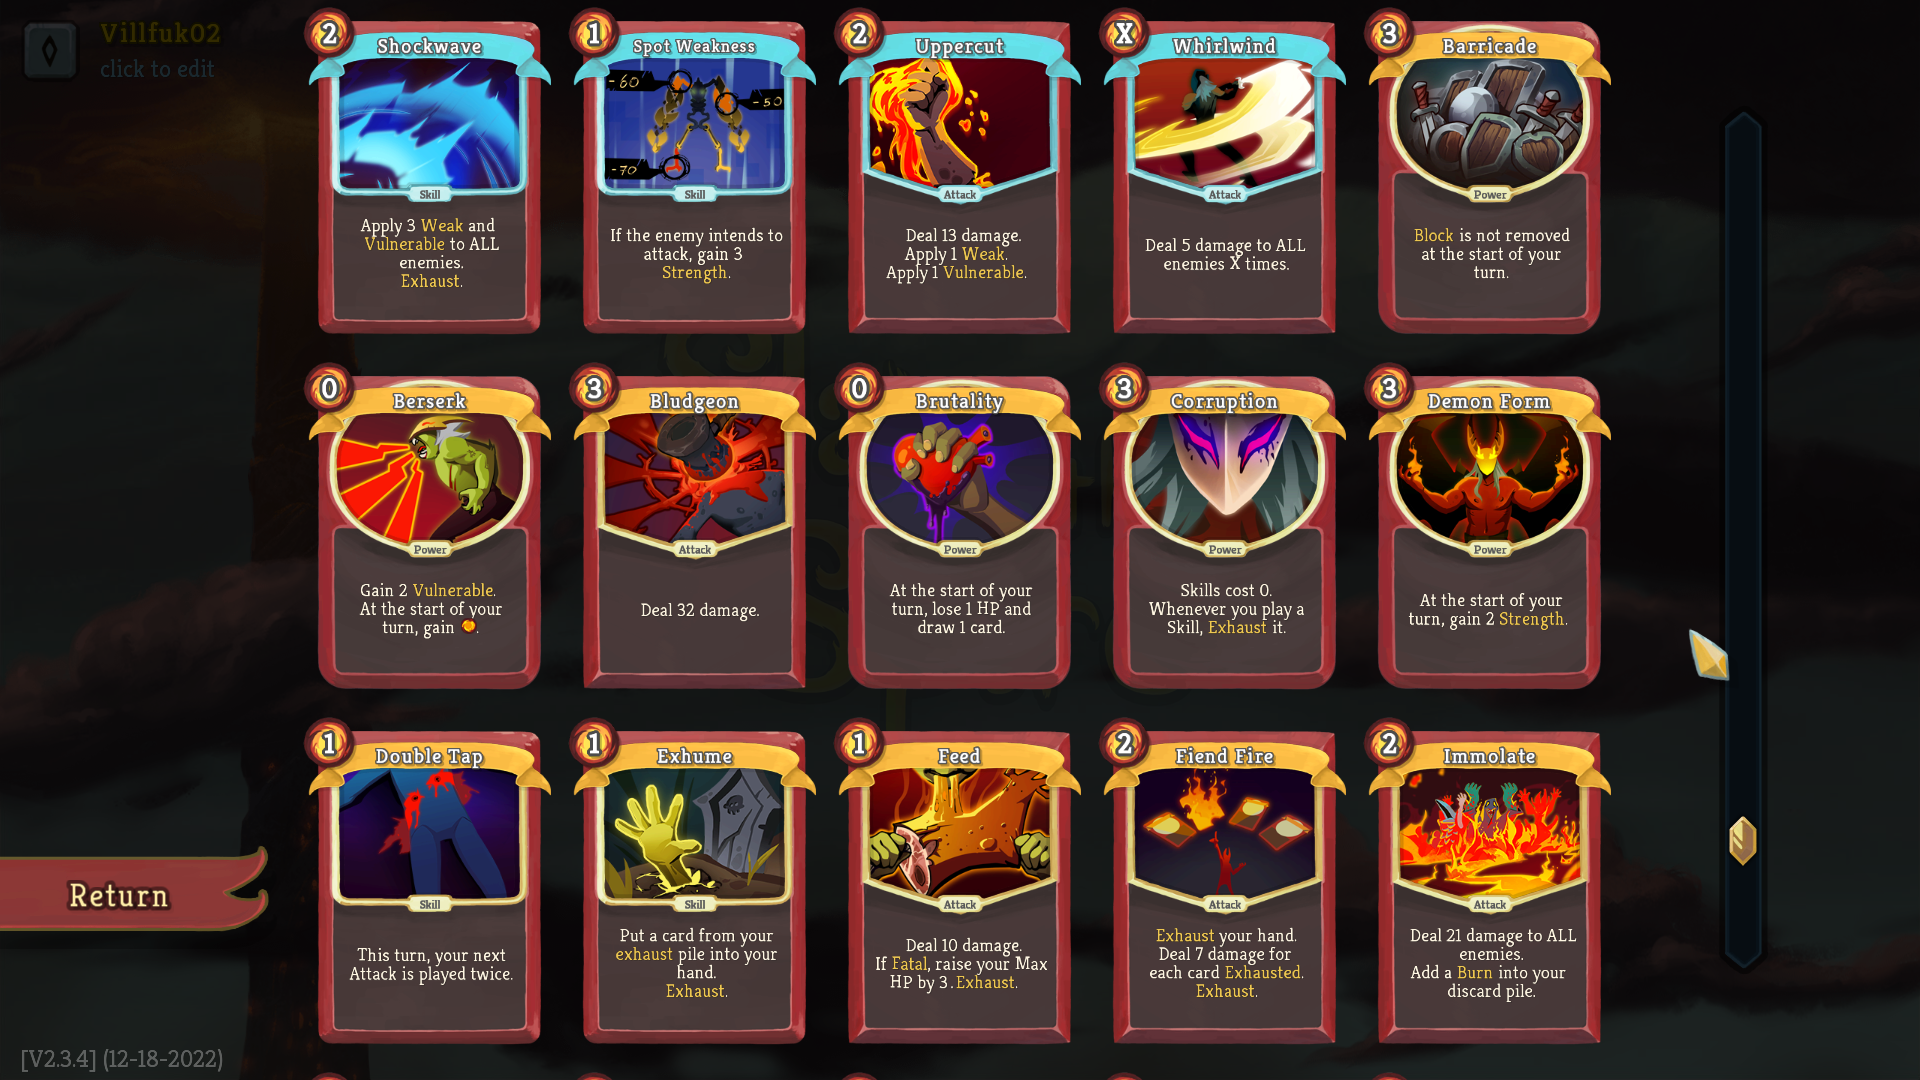
\includegraphics[width=0.8\textwidth]{img/Slay-the-Spire-Compendium.png}
    \caption{A small portion of the many interesting cards in Slay the Spire, viewed in the in-game compendium.}
    \label{fig:slay-the-spire-compendium}
\end{figure}

- PvZ --- the interactions are not so strong, but you have to combine the plants such that you have no weak spots --- cheap and expensive, for specific zombie types

\begin{figure}[htb]
    \centering
    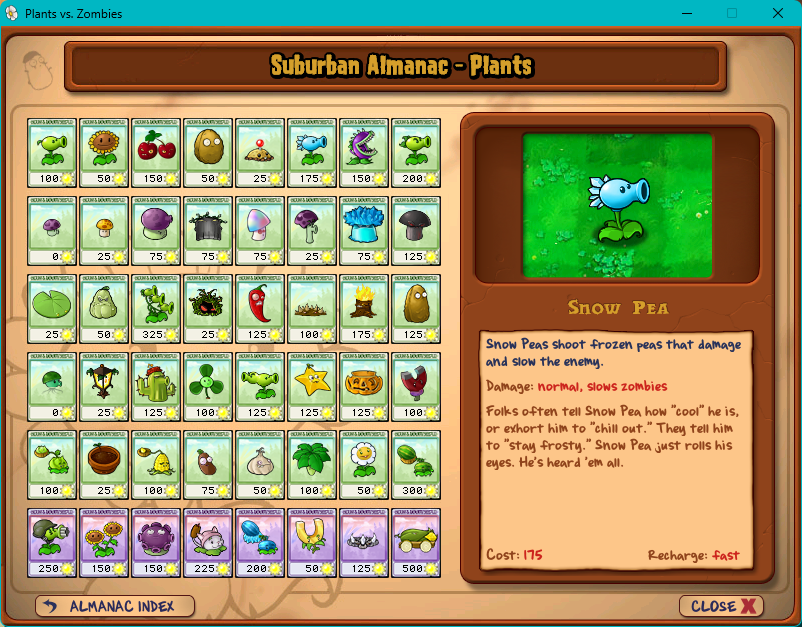
\includegraphics[width=0.8\textwidth]{img/Plants-vs-Zombies-Almanac.png}
    \caption{All the plants of Plants vs.\ Zombies in the in-game almanac.}
    \label{fig:plants-vs-zombies-almanac}
\end{figure}

- make blueprints that have unique effects that change the way you play

\subsection{Force Exploration} \label{sec:goal-force-exploration}

The player will have to use a different build every run.
We don't want the player to just find a single build that works and never explore anything new.
When the player is familiar with a build, it becomes stronger, since they know how to use it effectively.
This discourages them from trying other builds, because they can't use them so well, making them weaker.
Thus, we need to force the player to explore and make them put effort into learning other strategies.

- StS --- you have to explore different strategies because you get different cards every time, some enemies ensure you are prepared for everything and intentionally break some strategies

- characters

\begin{figure}[htb]
    \centering
    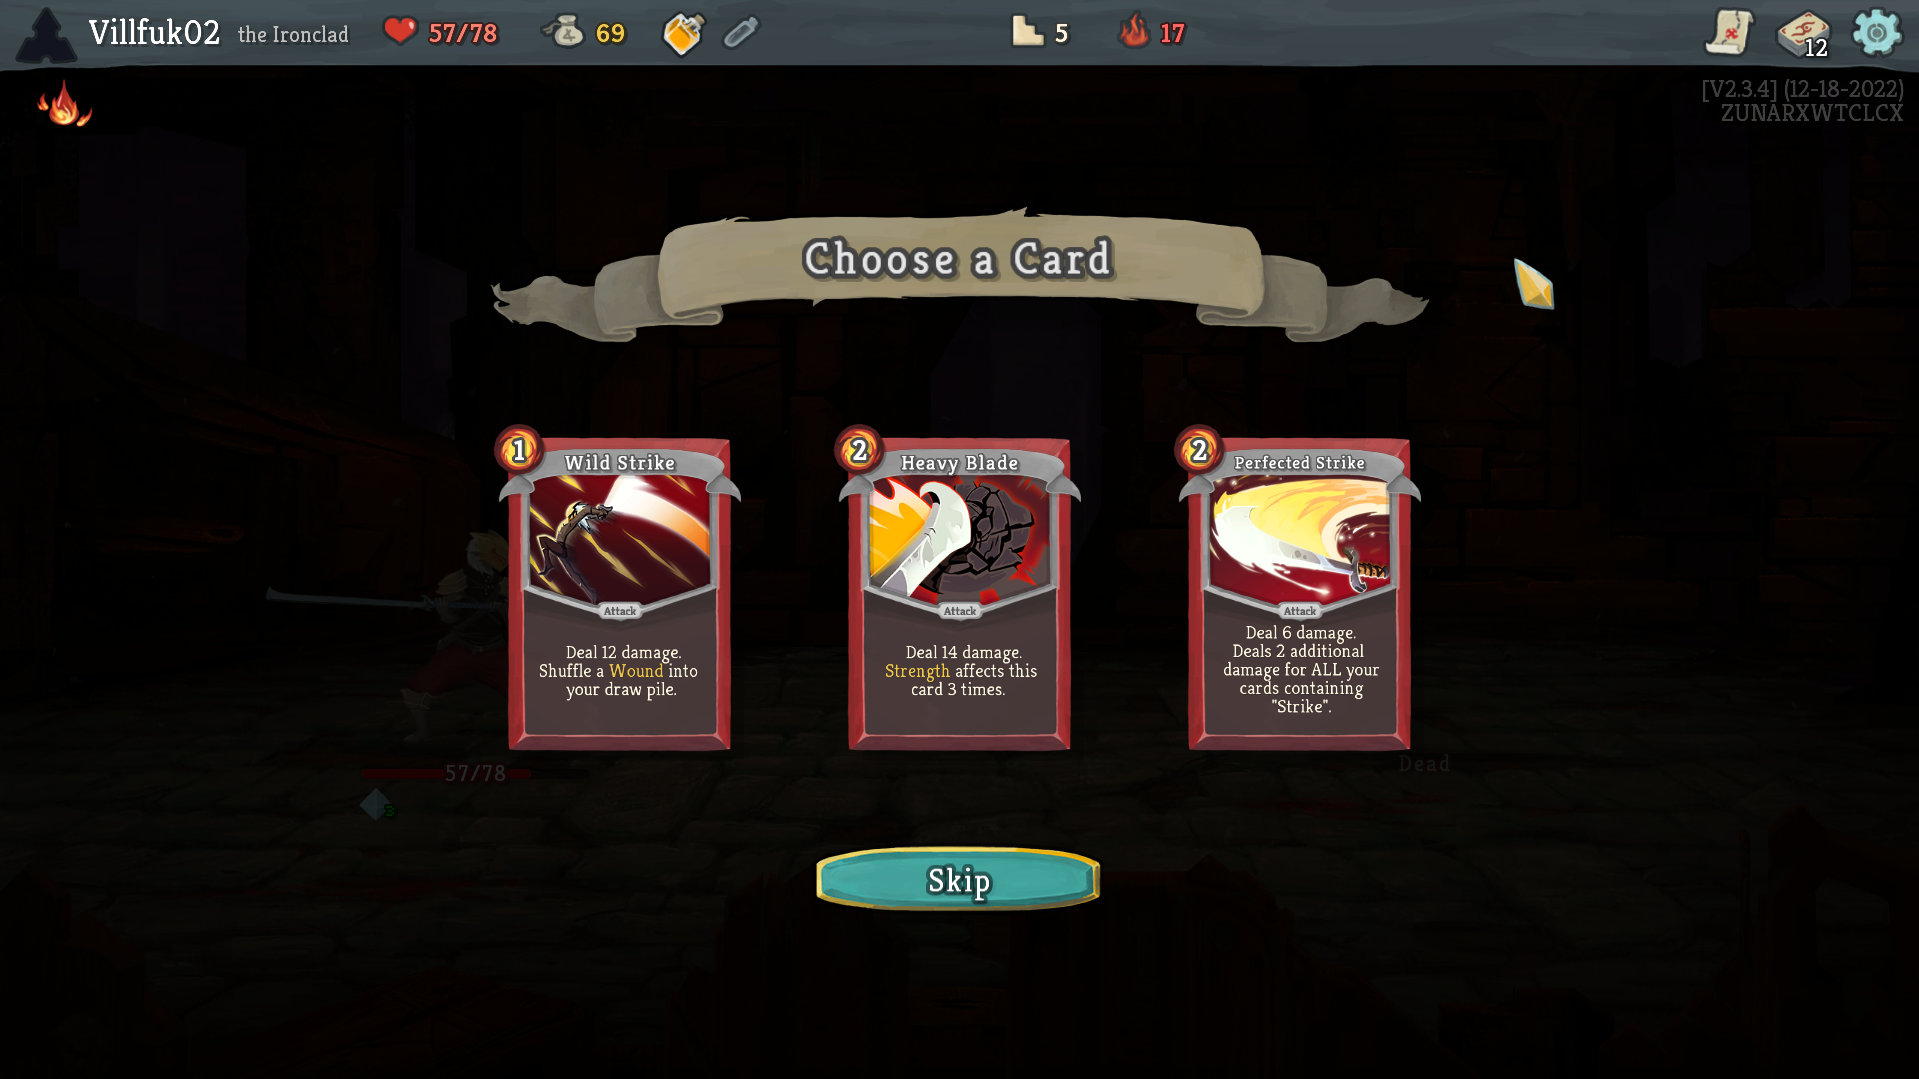
\includegraphics[width=0.8\textwidth]{img/Slay-the-Spire-Reward.png}
    \caption{Card reward screen in Slay the Spire. Here the player can choose on of three randomly selected cards to add to their deck.}
    \label{fig:slay-the-spire-reward}
\end{figure}

- PvZ --- you have to explore different strategies because you have to adapt to different zombies and level environments, not too deep; after the campaign, three seed slots are selected for you.

\begin{figure}[htb]
    \centering
    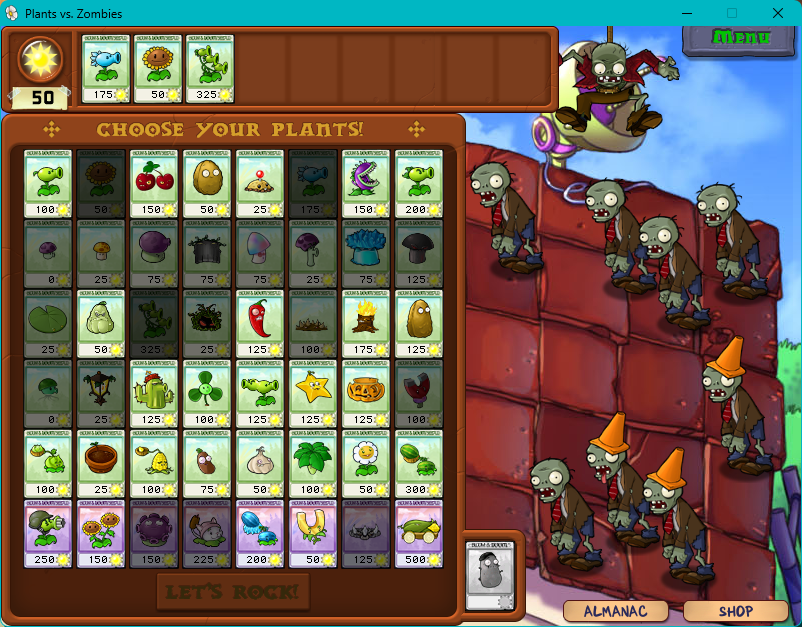
\includegraphics[width=0.8\textwidth]{img/Plants-vs-Zombies-Rooftop.png}
    \caption{Seed select screen in a rooftop level. Here, plants must be planted in flower pots, and most plants cannot shoot uphill.}
    \label{fig:plants-vs-zombies-roof}
\end{figure}

- choose from random blueprints, various attackers with abilities and terrain types

\subsection{Provide a Challenge} \label{sec:goal-challenge}

The player should always have some goal to work towards, just out of their reach.
If the game is too easy, the players will have no reason to think strategically or learn.
Always having a harder challenge to overcome will motivate the player to improve.

- StS --- not easy to beat; after you beat the game, you can play on a higher ascension

\begin{figure}
    \centering
    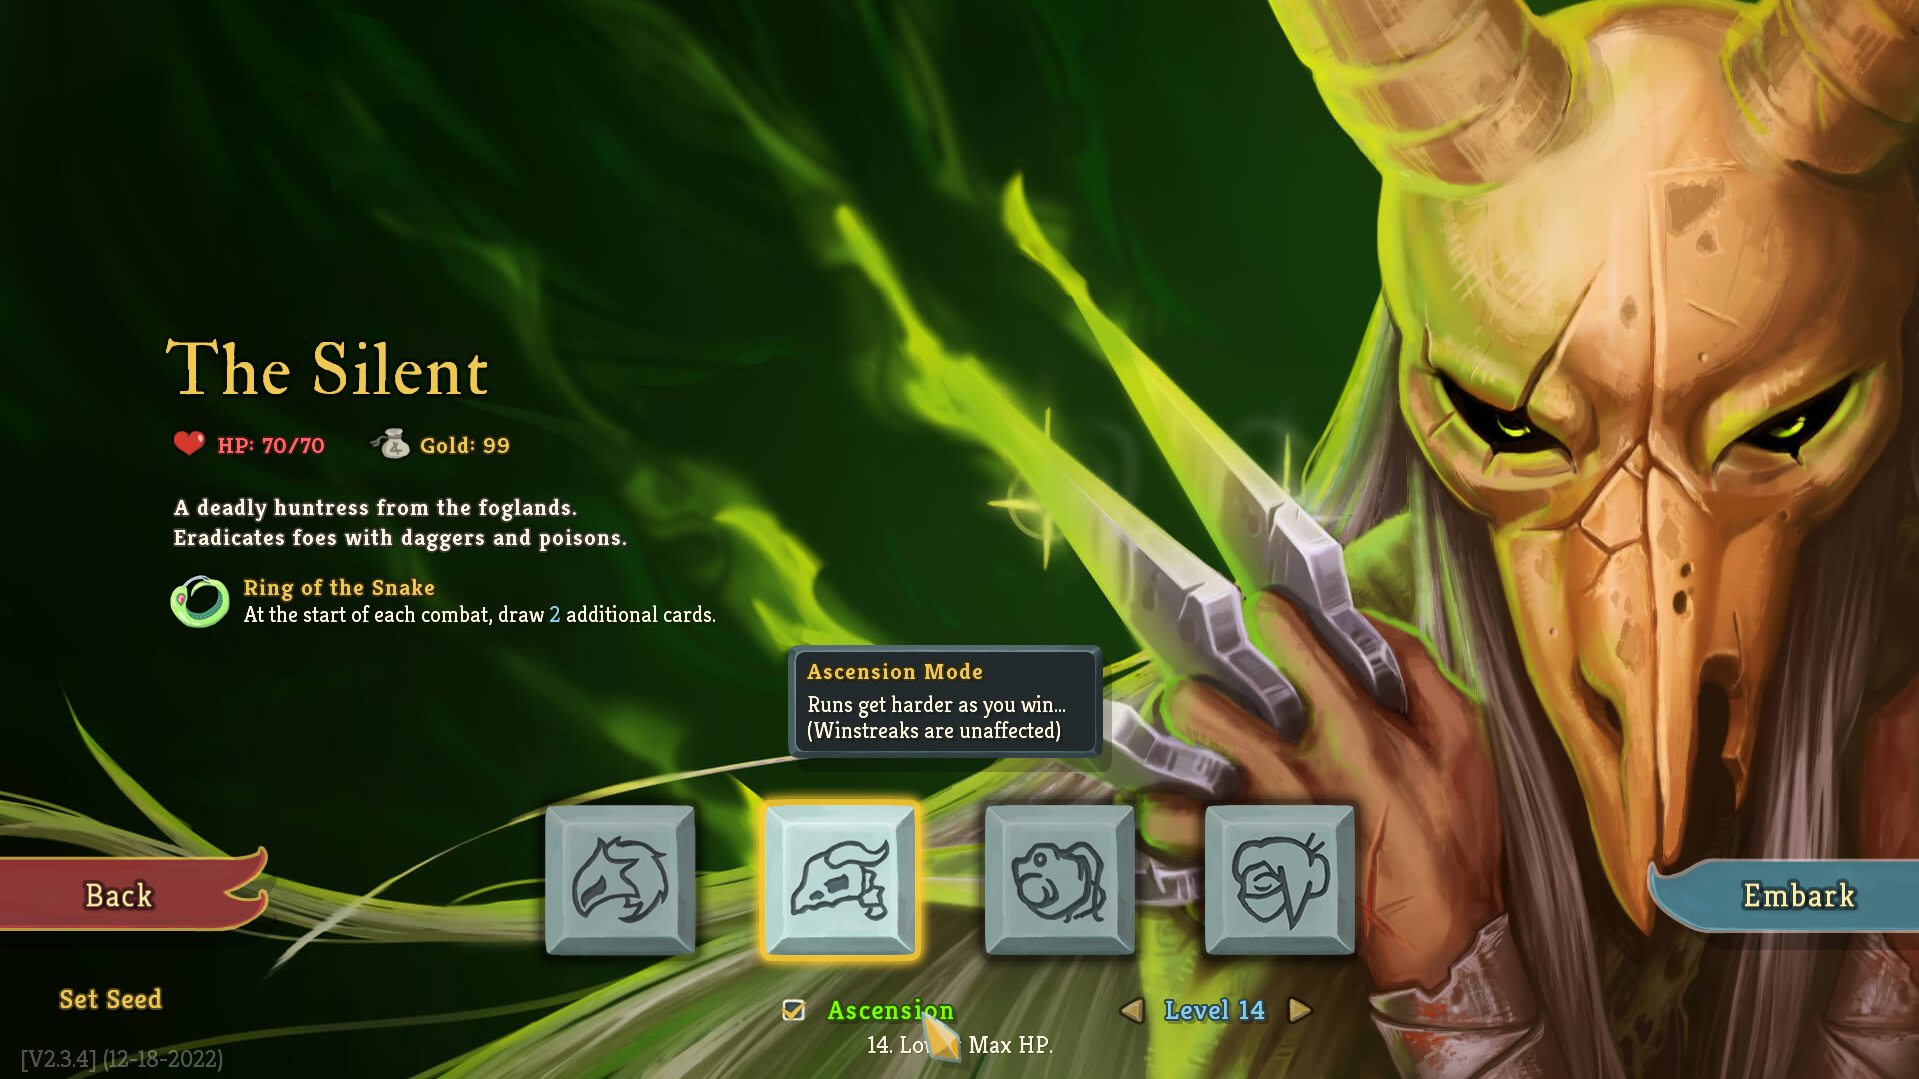
\includegraphics[width=0.8\textwidth]{img/Slay-the-Spire-Ascension.png}
    \caption{Character select screen in Slay the Spire. Here the player can also choose their ascension level, making the game harder.}
    \label{fig:slay-the-spire-ascension}
\end{figure}

- we will have something similar to StS

\section{Battle}

- build stuff, send waves, use abilities

\section{Attacker Movement}

- free movement with individual pathfinding X

- too unpredictable for the player --- The player needs to plan in advance in order to maximize the possibility to take calculated risks
- solution: visualize enemy paths --- Too many different paths - too much clutter; Still planning at most one wave in advance

- linear lanes (like in Plants vs.\ Zombies) X
- not enough space for interesting building placement

- paths based on your buildings X
- what if they block off the path?

- predefined paths \checkmark

- branching

- other qualities

\section{World}

- free placement X

- grid of tiles \checkmark
- more granularity, easier to develop intuition, same for attacker paths

- hexagons X

- squares \checkmark

- 3D \checkmark
- Simple and intuitive way to make the level itself more interesting
Some towers won't be able to shoot uphill or downhill - more interesting decisions for the player

- Terrain types (for now, just one)

- Obstacles

\section{Resources}

\xxx{for each subsection: what is it, why is it, how to acquire it, what are the constraints}

\subsection{Materials}

\subsection{Energy}

\subsection{Hull}

\section{Graphical User Interface}

\xxx{specify controls}

\subsection{Waves Left and Fuel}

\subsection{Hull}

\subsection{Wave Preview}

\subsection{Materials and Energy}

\subsection{Blueprints}

- what they represent

- limited number

- cost and cooldowns

- rarities

- make them unique

- lenticular design

\subsection{Info Panel and Selection}

- what it looks like and what's on it

- select blueprints

- select buildings

- select attackers

\subsection{Highlights and Range Visualization}

\section{Attackers}

- move, have health

- sizes

- special abilities - passive, repeating, reactive

\section{Buildings}

- how and when to build, one per tile

- special building have special abilities

- main types:

\subsection{Economic buildings}

-provide resources

\subsection{Towers}

- attack attackers

- range

- targeting

- projectile types

- damage types

\section{Abilities}

- used mid-wave

- usually instant effects

- free placement, global placement, tile placement, use on a building

\section{Camera controls}

- zoom to look closely, rotate so the terrain doesn't hide stuff

\section{Future Features}

- run structure

- map

- events and shops

- difficulty levels

- unlocks

\chapter{Analysis}

Now that we have described the game's design, in this chapter, we will explain the approach we took to implement it from a high-level perspective.
We will provide concrete details only for what will be implemented in the playable demo version, but as always, we will make many decisions based on the original vision of our game.

\section{Game Engine}

Game engines provide many important and useful systems for us, so we can focus on implementing the game logic.
For our game, we chose Unity because it offers all the features we need, and the author is already familiar with it.
There are many game engines we could have used, and the high-level decisions presented in this chapter would be still applicable.
However, in some sections we will use nomenclature that is specific to Unity, so we assume the reader is at least familiar with it.
More information is available in the official documentation~\cite{UnityDocs}.

\section{Procedural Generation}

As explained in the previous chapter, a lot of the game will be procedurally generated including the map of a run and each battle along the way.
From the player's perspective, all this and the rewards they receive will be randomized and unpredictable.
However, each run will have a single seed that deterministically decides all the \enquote{random decisions} the game makes.
Two runs with the same seed should look identical and if the player makes the same decisions and choices, the outcomes should be the same.
This allows the players to share seeds of the runs they found interesting and compare their skill in the same situations.
Furthermore, this is helpful for debugging, because it lets us easily reproduce any issue with the generation just by running it with the same seed.

We want to allow the player to save the game between battles.
Here, determinism is also useful, because it allows us to save just the seed of something that was generated, instead of saving it whole, which leads to simpler and smaller save files.

\subsection{Random Number Generators}

Randomized algorithms, like the ones we will use for procedural generation, depend on a \emph{random number generator} as their source of randomness.
A \textbf{random number generator} (or \emph{RNG}) produces a sequence of numbers that looks random and is unpredictable.
They are well explained in \citetitle{johnston2018random}~\cite{johnston2018random} by David Johnston.
Some RNGs use specialized hardware to generate truly random data using an external source of entropy, these are called \emph{true random number generators}.
However, we want a \emph{deterministic RNG}, also known as a \emph{pseudorandom number generator} (\emph{PRNG}).
These produce the random data using a completely deterministic algorithm, but unless we know the current internal state of the generator, the outputs still can't be predicted.
The initial state of a PRNG is called the \emph{seed}, and a generator will always generate the same sequence of outputs when \emph{seeded} with the same value.

Each query advances the generator's state, so the value a deterministic random number generator returns depends on the number of previous requests.
If we used one generator for generating everything, the outcomes of different systems would depend on the order they were generated in.
For example, when a player triggers some effect that uses randomness \emph{before} generating a level, the level would be different than if the player triggered the randomized effect \emph{after} the level was generated.
To remedy this, we will utilize a simple trick we call \emph{seed branching} all throughout the procedural generation.
Whenever we want more systems to be independent of each other, we create a new RNG instance for each system, and we seed them with each with a seed generated from the old RNG in advance.
For example, we will have a master RNG seeded with the seed of the run, from which we will generate the seeds for the map generator, reward systems, etc.
The map generator itself will generate the run map and then assign a new seed to each of the levels planned on the map, and so on.

We can determine what properties are required of the RNG we are going to use from our use-case.
First, obviously, the numbers generated by the generator should be random enough.
However, the RNG doesn't have to be cryptographically secure or pass strict statistical tests, since we aren't going to use them for cryptography or scientific simulations.
Since we will create many instances of the RNG, it should be lightweight and fast to initialize.
Some of them, for example the ones used by the reward system, will persist throughout the whole run, so we need an easy way to save the RNG's current state.
So, what options do we have?

Since we are using Unity, the first RNG that comes to mind is Unity class \texttt{Random}~\cite{UnityRandom}.
It is designed to be easy to use, but it is very limited~--- for example, we have access to only one instance of the class and the same instance is used for other systems within the game engine.
This is a dealbreaker for us, because we want to create more instances, and we want to have complete control over them to ensure determinism.

Another option that's on-hand is .NET \texttt{System.Random}~\cite{SystemRandom}.
According to the documentation, instantiating a random number generator is fairly expensive.
Furthermore, there are no methods to read and set the internal state of the generator.
This becomes a problem when we want to save the state of an instance to restore it later, for example when loading a save file.
We would have to serialize and deserialize the instance, which isn't a big problem, but it feels inelegant and inefficient.

Instead, we chose to go with a more straight-forward option~--- making our own RNG.
This way, we can make the generator have all the features we need.
There are many algorithms a PRNG can use.
Johnston describes in their book~\cite{johnston2018random} some most commonly used non-cryptographic PRNGs, namely:
\begin{itemize}
    \item Linear congruential generators (LCG),
    \item Multiply with carry (MWC),
    \item XORSHIFT,
    \item Permuted congruential generators (PCG).
\end{itemize}
All of these are random enough for our use-case, given we use the right parameter values, so we chose an LCG, because it seemed the most simple to implement.
In the article \citetitle{LCGTables}~\cite{LCGTables}, the author explains the statistical tests they used to measure the randomness of the LCGs and tabulates the best-performing parameter combinations.
From here we took the parameters for our LCG implementation.


\section{Path Generation}

- how to make paths with the required qualities?

\subsection{Initial Paths}

- inputs: hub position, path count, path lengths

- generate fixed number of paths with given lengths

- first pick *start points* from along the edges of the level (all paths end in the center of the level)

- choose randomly from positions with the correct parity (even / odd path length)

- spread them out by removing all positions near already chosen one

- then generate paths

- first trace it randomly, with bias away from the start and from path tiles

- simulated annealing

- there are just plans to make sure the paths exist and the terrain in a way that ensures that the paths are not blocked

\subsection{Final Paths}

- after terrain generation, the paths are traced for real

- guaranteed shortest length

- DFS, find all branches, but continue from bottom of the stack when a paths is found

\section{Terrain Generation}

- fractal noise X

- WFC \checkmark (don't forget to mention disadvantages)

\xxx{this is gonna be multiple subsections}

\xxx{illustrate with images (from the videos I made)}

- *slots* offset compared to *tiles*

- less distinct variants

- more control over transitions

- prepare *modules*

- generate grid of *slots*, mark them as *uncollapsed*

- each *slot* can become one of many *modules*

- the *modules* that can be placed in a given slot are its *domain*

- at the start each *slot* has all *modules* in its *domain*

- from the *domain*, compute all possible *boundary conditions*

- for example - there is a *module* in the *domain* with a cliff on its east boundary, so mark cliff to the east as possible

- mark all *slots* as *dirty*

- then repeat:

- propagate constraints

- for each *dirty slot*, until there are none:

- mark as *not dirty*

- find out which *modules* from its *domain* can be placed here and remove the rest from its *domain*

- decide only by neighbors' (orthogonal and diagonal) *boundary conditions*

- update *boundary conditions*

- if *boundary conditions* changed, mark all *uncollapsed* neighbors as *dirty*

- *collapse* a slot

- save the current *state* of all *slots* on a stack

- pick a *slot*

- pick one *module* from its *domain* at random

- weighted - provides control

- remove each other *module* from its *domain*

- update *boundary conditions*

- mark *uncollapsed* neighbors as *dirty*

- if a *slot* ends up with 0 *modules* in its *domain*, backtrack

- pop a prevoiusly saved *state* from the stack and revert to it

- remove the previously chosen *module* from the *domain* of the previously *collapsed slot*


- Which slot to collapse?

- fail fast approach

- prioritize slot with least options

- changed to slot with least entropy, because that's more accurate

- slots near most constraining modules were prioritized, making them more common and leading to repetitive terrain features

- better to just collapse a random slot

- in the end still weighted by entropy

- at first I tried to prefer slots with more entropy

- define overall structure first by sparsely covering the world, then fill in details

- often led to deep dead-ends with a lot of backtracking

- in the end, tiles with less entropy are preferred

- provide data

- Limited backtracking depth

- usually when more backtracking is required, the search would take too long and it's faster to restart the algorithm

- provide data

\section{Resources and Obstacles}

- after terrain generation, place blockers on tiles

- materials for the player to mine

- just rocks for variety - the player cant build on these

- set up as a few layers

- each stage has:

- one or more types of blocker (e.g. ore, small rocks, big rocks)

- *min* and *max* amounts

- *base chance* to place

- whether they can be placed on slanted tiles

- which surface Types they can be on (currently there is only one)

- *forces* - effect on chance based on already placed blockers

- for example: negative force with magnitude *m* from stage *s* means the chance to place a blocker on a given tile is decreased by *m/d*  for each blocker placed in stage *s*, where *d* is its distance from the considered tile

- for each stage:

- repeat until at least min blockers have been placed (in this stage)

- for each tile without a path or blocker (in random order):

- if random number between 0 and 1 < modified chance:

- place the blocker of the given type

- if there are max blockers (placed in this stage), end the stage

- scattering models

- unity physics engine X

- parallel

For the blockers, I didn't want repetitive obstacle models, so they are generated proceduraly by scattering many simpler models (decorations) on each tile

- first compute weights based on various factors (images!!!)

- distance to path

- height

- distance to other blockers

- customizable thanks to modular approach

- then scatter decorations in stages, each stage again having one type of decoration and many parameters

- for each tile in random order repeat x (specified for this stage) times:

- pick a random position within it

- calcualte the weight at this position (based on settings)

- check that it is greater than some threshold (based on settings)

- calculate the minimum distance to other decorations (from weight, based on settings)

- check that the position is far enough from other decorations

- calculate the decoration size (from weight, based on settings)

- place the decoration on this position, with the given size

\section{Terrain Types}

- what information is tied to the type

- why txt (inspector was not as legible)

\section{World Builder}

- builds the world from the generated data, it needs to be done in the main thread

\section{Attacker Wave Generation}

- creates a randomized plan of waves

- two types of waves

- combine different attackers in sequence

- combine different attackers in parallel (only possible with multiple paths, rarer)

- each wave gets some throughput budget and buffer

- each attacker has a given cost

- when planning a wave, select attackers and spacing, such that the througput budget is exceeded

- for each attacker subtract the throughput overshoot from buffer

- fit such that as much of buffer gets used without going over

- branching

\section{Simulation}

- use fixed updates for game logic

- why?

- 20Hz = fixed time step 0.05s

- options to speed up or possibly pause - changing fixed update rate - not yet implemented

\section{Visuals and Interpolation}

- interpolate positions and visuals on Update

- many visuals are game-speed agnostic     - TODO: use unscaledDeltaTime

- I thought about some custom mini-framework for this, but many of the simulated variables the visuals are based on should be handled on case-by-case basis

\section{Attacker Targeting}

- Towers use it to acquire targets

- handles which Attackers are in range and which one is chosen as the current target

- can require line of sight to the enemy

- different targeting types

- rotation

- heights

- possibly ensure a trajectory

- preferred target (configurable)

- composite colliders

\section{Range Visualization}

- IMAGES!!

- Draw the range on the terrain mesh

- Draw on which parts of paths will Attackers be targeted

- green - all sizes

- yellow - only large

- Terrain shader uses compressed texture format instead of raw texture

- Options:

- quadrant compression format, 2bytes per node

- less CPU time, because the data is already in this format

- up to 48KiB per frame

- more GPU time

- 256x256 texture, 1byte per pixel

- more CPU time

- 64KiB per frame

- fast on GPU

- only 1 channel - cannot interpolate

- mipmaps -> one additional state

- less CPU time

- 33\% more data

- more pixels per byte

- possible future optimization

- less data

- more difficult indexing and stuff both on CPU and GPU

- interpolation could work with more than one channel and without mipmaps

\section{Game Commands}

- we want various components to modify how other components function

- examples

- also react to events as a bonus

\section{Blueprints}

- separation of stats from behavior

- why are they implemented this way

\subsection{Attacker Stats}

- blueprints for attackers

\subsection{Dynamic Descriptions}

- explain what things do and their stats

- attackers and blueprints

- dynamically reflect the changes made by other components

\chapter{Developer Documentation}

In this chapter we aim to describe the implementation of the demo version of our game.
In the first section~\ref{sec:docs-proj} we describe the overall structure, and in the later sections we go into more detail about the individual parts.
Section~\ref{sec:docs-data} describes what goes on from the application start to the end, including all procedural generation, but not what happens during a battle.
We will focus on battles first, in section~\ref{sec:docs-battle}.

\section{Project Structure}\label{sec:docs-proj}

In Unity, each project is composed of individual scenes.
The scenes contain game objects to which are attached scripts that provide their behavior.
These are all saved in the project's asset folder, along with all other resources like prefabs, models, materials, textures, sounds and more.
They are separated to folders based on their type, for example all scenes are in the \emph{Scenes} folder.

In addition to the project assets, an important part of the project are the project settings.
However, these are all mostly set to their default value from the standard \emph{3D (Built-in render pipeline)} project template.
The settings that were changed are all uninteresting adjustments that an experienced Unity user would expect us to configure how we did, based on the explanation of our project provided in this chapter and chapter~\ref{analysis}.
These include for example settings in categories \emph{Tags and Layers}, \emph{Physics} and \emph{Player}.

\subsection{Scenes}\label{sec:docs-scenes}

The demo version of our game is composed of 5 scenes.
We provide a brief summary of each, but we will describe them in more detail later.
This summary will be useful for the rest of the chapter, allowing us to see which parts of the game occur chronologically after other parts.
For convenience, the transitions between the scenes are shown in figure~\ref{fig:scene-transitions}.

\begin{center}
    \captionsetup{type=figure}
    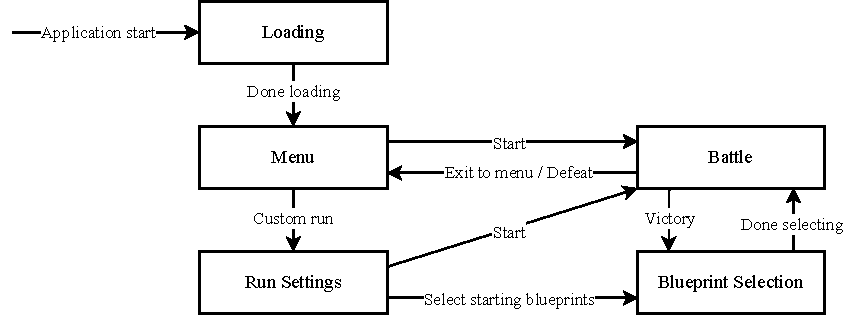
\includegraphics[width=0.9\textwidth]{img/Scene transitions.pdf}
    \caption{Scene transitions.}
    \label{fig:scene-transitions}
\end{center}

\begin{itemize}
    \item \textbf{Loading} is the first scene that gets loaded when the game starts.
          This scene contains only scripts that load data and game objects that persist throughout the entire lifetime of the application.
          After the loading is done, this scene transitions to \emph{Menu}.
    \item \textbf{Menu} contains the game title, and a button to start a run, a button to set up a custom run, and a button to exit the game.
          The start button takes the player to the \emph{Battle} scene, whereas the custom run button leads to the \emph{Run Settings} scene.
    \item \textbf{Run Settings} lets the player customize the run by selecting a custom seed or by opting to select their starting blueprints.
          There is also a button that lets the player play again the in-game tutorial.
          Starting a run from here also takes the player to the \emph{Battle} scene, unless they chose to select starting blueprints in which case they go to the \emph{Blueprint Selection} scene.
    \item \textbf{Battle} is the scene where the battles take place.
          First, the world is procedurally generated.
          Then the player plays one level of the game, until they win the level or lose.
          If they lose, their only option is to return to \emph{Menu}.
          When they win, they continue to the \emph{Blueprint Selection} scene.
    \item In \textbf{Blueprint Selection}, the player is shown their current blueprints and new blueprints to choose from.
          When they finish choosing, they continue to the next \emph{Battle}.
\end{itemize}

\subsection{Scripts}\label{sec:docs-scripts}

Most game object exist only within one scene, but some persist between scene transitions.
Each battle happens in one scene, but it still contains multiple separate systems.
This means that we cannot judge the structure of the project just by the scenes.
The structure of \emph{Scripts} folder should be more informative.
The scripts are divided based on their function into these 6 subfolders:
\begin{itemize}
    \item \textbf{BattleSimulation}~--- game logic of the systems present in a battle. Used in the \emph{Battle} scene.
    \item \textbf{BattleVisuals}~--- logic for the visuals during a battle like animations, particle effects and the user interface. Used in the \emph{Battle} scene.
    \item \textbf{Data}~--- parsing and loading data from the disk in the \emph{Loading} scene. It also contains singleton classes the data is loaded into to be used by other scripts in the application.
    \item \textbf{Game}~--- systems and concepts that are present outside battle, across multiple battles or throughout the whole application runtime.
    \item \textbf{Utils}~--- various utility functions and data structures used throughout the project.
    \item \textbf{WorldGen}~--- procedural generation of the world for each level, used in the \emph{Battle} scene.
\end{itemize}

Each of these folders is split further into more subfolders, each usually representing one game system.
The scripts are also separated into namespaces which exactly match the folder structure.
We also usually place one assembly definition asset in each folder, which make unity separate these scripts into different assemblies in the project solution.
This is done shorten compilation times because the codebase is rather large.

We will further describe the scripts in the subfolders in the following sections, but first we'd like to mention the function of the scripts \mono{SceneController} and \mono{SoundController} in the \emph{Game/Shared} script folder.
Both these scripts are attached to game objects in the \emph{Loading} scene which persist between scenes throughout the whole application lifetime.
They are both singletons that provide some functionality for other scripts using static functions.
The \mono{SoundController} lets other scripts play stationary sound effects, and is used all throughout the application.
\mono{SceneController} lets other scripts seamlessly change scenes by fading out the screen to black, then changing the scene, and fading back in once the new scene is loaded.

We would also like to mention that in the code, in \mono{MonoBehaviour} scripts, we use some conventions that might seem odd to programmers who don't use Unity.
For example, many private fields have the attribute \mono{[SerializeField]} which makes them show up in the Unity editor in the inspector.
This lets us save the values of these fields as a part of the scene, instead of initializing them in code.
We can also inspect the value of these fields at runtime in the Unity editor.
Since properties don't show up in the inspector, we use public fields in many places where it would be more appropriate to use a property with a public getter and a private setter.

\subsection{Third-Party Assets}
In the project, we use some assets that were not created by the author of this thesis in addition to the Unity game engine.
We would like to acknowledge and disclaim these assets here:
\begin{itemize}
    \item The Unity package \textbf{UI Soft Mask} by \emph{mob-sakai}~\cite{SoftMask}.
    \item We adapted the implementation of a \textbf{Priority Queue} from the \emph{.NET Platform}~\cite{PriorityQueue}.
    \item We also adapted an \textbf{Editor Init} script by \emph{Z4urce}~\cite{EditorInit}, used to select the scene to load when we run the game in the Unity editor.
    \item And a function for calculating the number of set bits in an \mono{int}, or \textbf{Hamming Weight}, from this \emph{stack overflow} answer~\cite{PopCount}.
    \item The font used for all text in the game is \textbf{Open Sans} by the \emph{Open Sans Project contributors}~\cite{OpenSans}.
\end{itemize}

\section{Battle}\label{sec:docs-battle}

In this section, we discuss the systems that come into play during a battle.
When the \emph{Battle} scene is loaded, some scripts generate the world and some other scripts initialize various parts of the scene.
Throughout this, the screen is faded out to black.
It fades in and lets the player interact with the scene only after all the initialization is done.

From the player's perspective, after the game fades in, the battle alternates between the building phase and the wave phase, as shown in figure~\ref{fig:battle-phases}.
In the building phase, the player can build buildings.
When they start the next wave, the game goes to the wave phase, where the player can use abilities, but cannot build buildings.
Once all attackers are killed, the game goes back to the building phase.
This repeats until the player wins this level or lose the game.

\begin{center}
    \captionsetup{type=figure}
    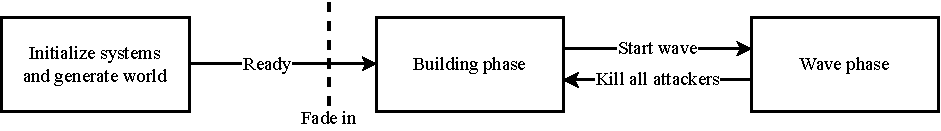
\includegraphics[width=0.8\textwidth]{img/battle scene phases.pdf}
    \caption{\emph{Battle} scene phases.}
    \label{fig:battle-phases}
\end{center}

We will explain the initialization and procedural generation in section~\ref{sec:docs-world-generation}.
In this section, we'll describe only the processes involved in the gameplay.
First we'll explain the game logic, and then the visualizations used to communicate information to the player.

To most systems in involved in the battle, it doesn't matter if the game is currently in the building or wave phase, they behave the same at all times.
Only few things change when a wave starts or ends, which we describe in section~\ref{sec:docs-waves}.

\subsection{Scene contents}\label{sec:docs-battle-scene}

Before we explain what goes on during a battle, we should introduce the contents of the battle scene.
When loaded, the \emph{Battle} scene contains only the UI, and various singleton objects with scripts that each take care of one game system.
We will explain these when they become relevant.

During the procedural generation and initialization, more game objects are created in the scene and various scripts are initialized with data.
For example, the results of the world generation are stored in the \mono{WorldData} singleton script.
The world terrain is created in the scene under the \emph{World} game object, including the obstacle models and visualization of the attacker paths.
Also, an instance of the \emph{Tile} prefab is created for each world tile, and references to the tiles are also stored in \mono{WorldData} script for easy access.
For the rest of this section, we assume the scene is already initialized and ready for the player's inputs.

During the battle, there are also some game objects which persist between scenes and don't originally come from the \emph{Battle} scene.
These are the \mono{SceneController} and \mono{SoundController} we introduced in section~\ref{sec:docs-scripts}.
Additionally, there is \emph{Run Persistence} game object, which contains scripts that persist throughout the player's run.
The only script relevant during battle it has is \mono{RunPersistence}, which keeps track of the player's blueprints and hull.
We will describe it in more detail in section~\ref{sec:docs-run-persistence}.

\subsection{Selecting World Objects}

During the battle, one of the most important things the player can do is to build buildings or use abilities.
To do that, the player first needs to select the blueprint they want to use.
The \mono{SelectionController} keeps track of what objects the player selects or hovers over.
In this subsection, we will illustrate the \mono{SelectionController}'s function by explaining what happens when the player selects objects within the game world.
Selecting and placing blueprints is more complicated, and it will be explained in the next subsection~\ref{sec:docs-place-blueprint}.
The game also visualizes which objects are currently selected or hovered, and it shows additional information on the info panel.
This is ultimately the reason why the player would select a world object.
These visual components will be explained in section~\ref{sec:docs-highlights}, and how the info panel works is described in section~\ref{sec:docs-info-panel}.

In the world, the only selectable objects are tiles and attackers.
When the player selects a building, they have in fact selected the tile the building is built on.
Every frame, the \mono{SelectionController} performs a raycast to determine which selectable object is the cursor over, if any.
The selectable objects have a game objects with a collider on the physics layer \emph{Selection} and a \mono{Selectable} script.
If a selectable world object is hovered over, a reference to its \mono{Selectable} script is saved in the \mono{SelectionController} as currently hovered.
Whenever the currently hovered object changes (even to \emph{null}), the info panel is notified to show information about the hovered object (or to hide).

When the player clicks while an object is hovered, it is selected:
The \mono{selected} field in the \mono{SelectionController} is set to the hovered object and the info panel is notified.
While something is selected, the \mono{SelectionController} still updates which object is hovered.
When the player deselects the object, the field is unset, and again, the info panel are notified.

\subsection{Selecting and Placing a Blueprint}\label{sec:docs-place-blueprint}

Let's start with an example of what happens when from the player's perspective when they place a blueprint:
The player clicks on a blueprint of a tower in the blueprint menu.
It is now selected.
Then, they hover over the tile they want to place the tower on.
The game shows a visualization of the range the tower would have if it was placed there.
We say the selected blueprint is set up as if it was placed there.
Finally, the player clicks to place the tower on the selected tile.

We can see that each of the player's actions had an effect on the state of the selection.
In this section, we'll take a look at what happens in response to each of the player's actions in order to achieve this behavior.
For reference, the possible selection states and action that transition between them are shown in figure~\ref{fig:selection-states}.
Each arrow represents what the player can do in the current state and what is the new state after the action is performed.
Few actions are show with blue arrows instead of black.
These are still actions the player can take, but in the code, they are performed as a deselection followed by a selection.

\begin{center}
    \captionsetup{type=figure}
    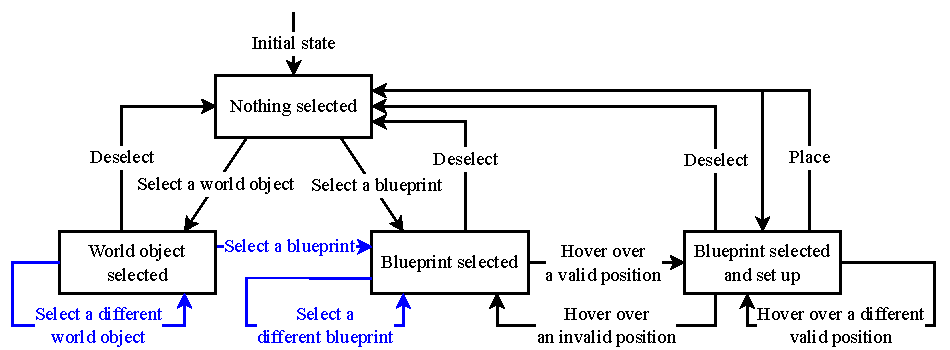
\includegraphics[width=\textwidth]{img/selection states.pdf}
    \caption{Selection states.}
    \label{fig:selection-states}
\end{center}

We have already explained what happens when a world object is selected or deselected, but things are a bit more complicated with blueprints.
We will now explain each of the remaining actions in the diagram.

\head{Selecting a Blueprint}{}
A blueprint can be selected by clicking on it in the blueprint menu user interface (see section~\ref{sec:design-blueprint-menu}) or by pressing a number key on the keyboard that corresponds to its position in the blueprint menu.
Either way, the \mono{SelectionController} gets only the blueprint's index in the blueprint menu.
If this index corresponds to the currently selected blueprint, it gets deselected.
But now, we'll look at what happens when a blueprint gets selected.
During this, the \mono{SelectionController} interacts with other scripts.
Figure~\ref{fig:placing-blueprint} contains a sequence diagram for reference.

First, the \mono{SelectionController} obtains the actual blueprint at the given index from the \mono{BlueprintMenu}.
Then it takes the prefab associated with this blueprint and instantiates it.
Each blueprinted object prefab has on it two scripts that are relevant for us right now:
A script derived from \mono{Placement}, which decides where the blueprint can be placed.
And a script derived from \mono{Blueprinted}, which handles the behavior of the blueprinted object when placed in the world.
For example, the \emph{Budget Sentry} has the script \mono{SimpleBuildingPlacment} for placement and its behavior is implemented by the script \mono{BasicProjectileTower}.

After instantiating the prefab, the \mono{SelectionController} saves a reference to its \mono{Placement} script which signifies that this is the currently selected object.
It then initializes the \mono{Blueprinted} script by giving it a copy of the original blueprint.
Similarly to selecting a world object, it notifies the info panel to show the relevant information.
This is not shown in the sequence diagram to avoid clutter.

\head{Setting Up the Blueprint}{}
We want to accurately preview the effects a blueprint will have, or how it will be affected by other buildings once placed.
To do this, we need to position the blueprinted object in the world as if it actually was placed.
On every update, the \mono{SelectionController} tells the \mono{Placement} to set up the object as if it was placed in the position the player currently hovers over.
The \mono{Placement} returns whether the setup changed from the last frame, and if it did, the \mono{SelectionController} also notifies the \mono{Blueprinted} script.

It is possible that the current position is not a valid placement for the blueprint.
In that case, the \mono{Placement} marks the setup as invalid.
This is represented in figure~\ref{fig:selection-states} as the state \enquote{Blueprint selected}.
However, for the \mono{SelectionController}, there is no distinction between a valid and invalid setup.
From its perspective, the states \enquote{Blueprint selected} and \enquote{Blueprint selected and set up} are just one state.
To the player, they are pretty distinct, because the various visualizations behave differently based on whether the current placement is valid or not, and they communicate the difference to the player.
How these visualizations work is explained in section~\ref{sec:docs-highlights}.

\begin{center}
    \captionsetup{type=figure}
    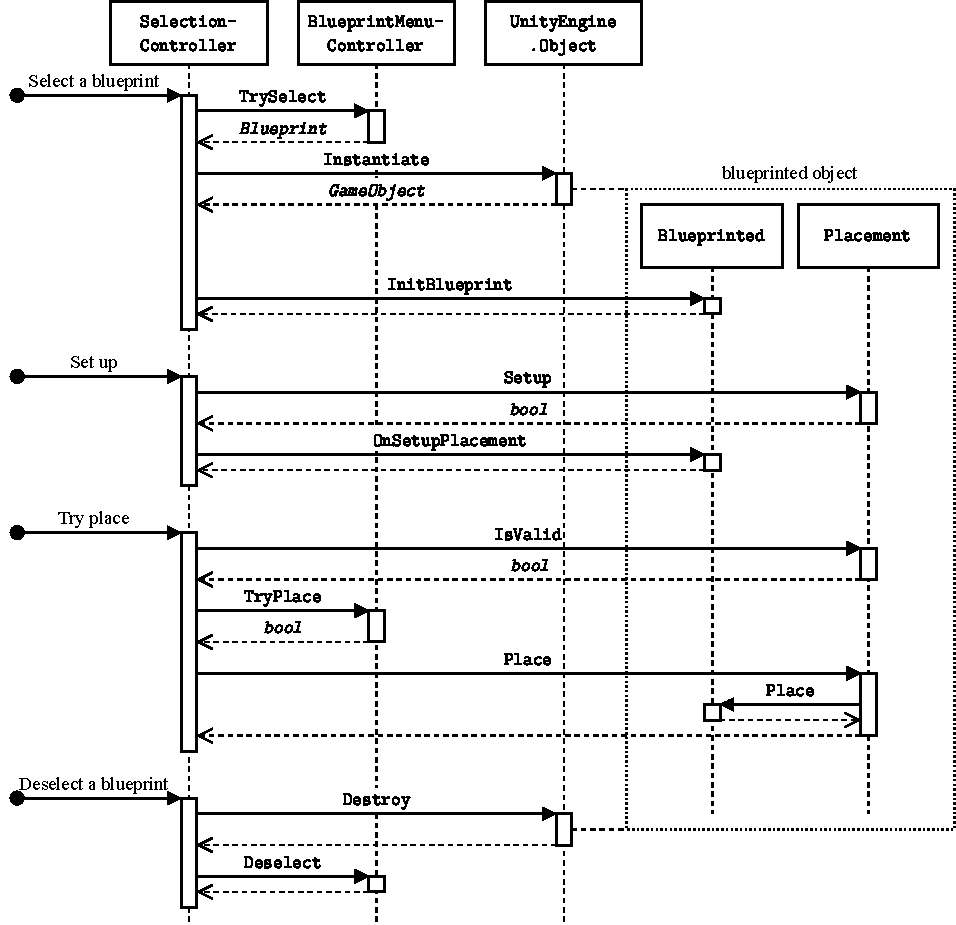
\includegraphics[width=\textwidth]{img/placing a blueprint.pdf}
    \caption{Sequence diagram of events related to placing a blueprint.}
    \label{fig:placing-blueprint}
\end{center}

\head{Placing the Blueprint}{}
When the player clicks to place the selected blueprint, the \mono{SelectionController} first asks the \mono{Placement} if this position is valid.
If it is, the \mono{SelectionController} asks \mono{BlueprintMenu} to try to place the blueprint.
This only means that the \mono{BlueprintMenu} checks if the player can afford the cost and that the blueprint isn't on cooldown.
If this succeeds, the \mono{BlueprintMenu} invokes a command to subtract the cost of the blueprint from the player's resources, and it makes the blueprint go on cooldown if applicable.

If the blueprint cannot be placed, the \mono{SelectionController} just plays an error sound to provide feedback to the player.
Otherwise, it calls the \mono{Place} method on the blueprinted object's \mono{Placement}.
Then the \mono{SelectionController} deselects the blueprint.
However, in figure~\ref{fig:selection-states} the \enquote{Place} action forks and leads to two different states.
This just signifies that after placing an ability, the blueprint gets automatically selected again.

After being actually placed, the \mono{Blueprinted} script enables the visual parts of the blueprinted objects, but the rest is left up to the implementation of the given object.
Usually, their initialization includes registering some modifiers and reactions to modifiable commands (see section~\ref{sec:analysis-modifiable-commands}).
For example, most production blueprints produce resources every turn, so they register a modifier to the modifiable query which determines the production per turn displayed to the player.
They also register a reaction to the event signifying that a wave has ended, because they produce the resources specifically after every wave.

\head{Deselecting the Blueprint}{}
If the selected blueprint gets deselected without placing it, the blueprinted object gets destroyed and the \mono{BlueprintMenu} is notified that the blueprint is no longer selected.
This can also be seen in figure~\ref{fig:selection-states}, but note that the exact sequence of events shown in the diagram is invalid.
It is not possible to deselect a blueprint after it has already been placed.

\head{Hovering over a Blueprint}{}
We would also like to mention how we handle hovering over a blueprint in the blueprint menu, because it is different from hovering over a selectable world object.
In fact, the \mono{SelectionController} doesn't know when the player hovers over a blueprint.
As far as it knows, the player doesn't hover over anything.
The blueprints in the blueprint menu detect the hover on their own and react to the hover accordingly, including notifying the info panel.
The script that makes this work is the \mono{BlueprintDisplay} script on each of the blueprint menu items.
This is done this way, because the blueprint display prefabs are also used in the \emph{Blueprint Selection} scene, where they behave the same.

\subsection{Player State}

Another important singleton script in the \emph{Battle} scene is the \mono{PlayerState}.
Compared to the \mono{SelectionController}, its function is much simpler.
It keeps track of the player's energy, materials and fuel, and if the battle has been won or lost.
Other scripts can use its static modifiable commands to add or spend resources.

Once the fuel amount reached the fuel goal for this level, it invokes its modifiable command \mono{WIN\_LEVEL}.
In reaction to this, the \mono{OverlayController} shows the victory overlay with a button to proceed to the next level.
What happens next is explained in section~\ref{sec:docs-run-persistence}.

\subsection{Attacker Waves}\label{sec:docs-waves}

The \mono{WaveController} script controls what happens during a wave.
It interacts with several other scripts, which we'll describe in the following paragraphs.
For reference, we've lillustrated these interactions in figure~\ref{fig:wave-controller-interactions}.
The diamonds are modifiable commands or events, and for their interactions, we use a convention similar to the diagrams in section~\ref{sec:analysis-modifiable-commands}.

\begin{center}
    \captionsetup{type=figure}
    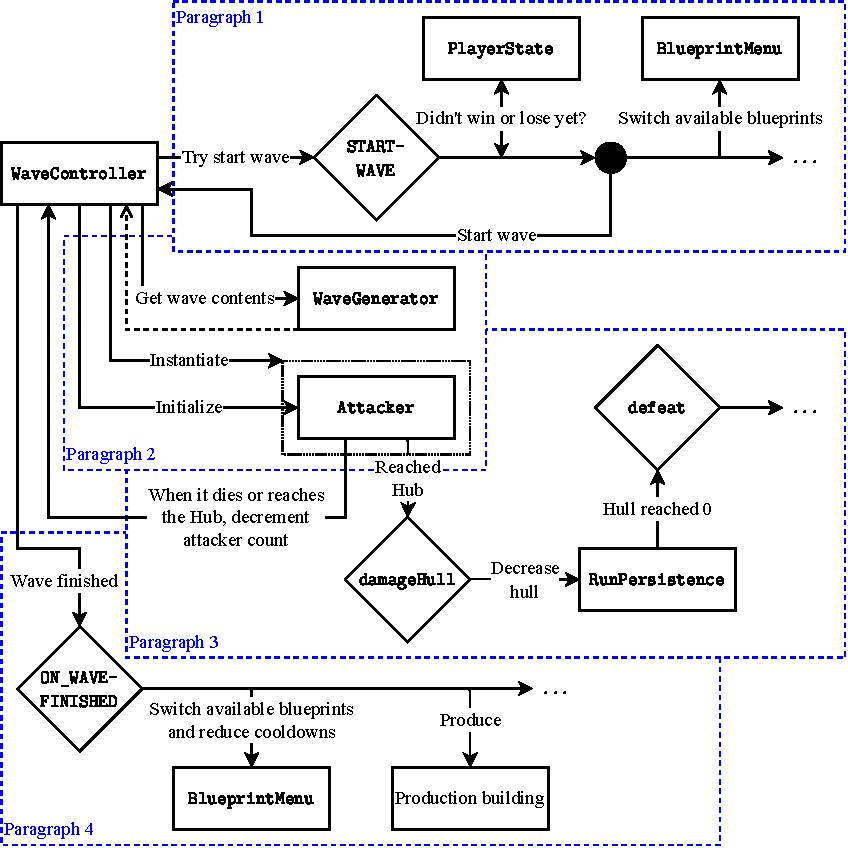
\includegraphics[width=\textwidth]{img/wave controller connections.pdf}
    \caption{Interactions of \mono{WaveController} with other scripts.}
    \label{fig:wave-controller-interactions}
\end{center}

\paragraph*{(1)}
When the player requests to start a new wave, the \mono{WaveController} invokes the \mono{START\_WAVE} modifiable command.
This command has a modifier registered by \mono{PlayerState}, which cancels the command if the battle has been won or lost.
Various scripts react to this command, for example the \mono{BlueprintMenu} changes which blueprints are available from buildings to abilities.

\paragraph*{(2)}
When the wave is started, the \mono{WaveController} requests the contents of the wave from the \mono{WaveGenerator}, and it starts spawning the specified attackers.
To spawn an attacker, it instantiates the prefab specified by the attacker stats, and it initializes the attacker's \mono{Attacker} script.
The attacker then moves and behaves on its own, as implemented in its \mono{Attacker} script.

\paragraph*{(3)}
The \mono{WaveController} does not keep track of the attackers, only their count.
Whenever it spawns an attacker, it increments the count, and whenever an attacker dies or reaches the Hub, the count is decremented.
Once all attackers have been spawned and there are no attackers left in the world, the wave ends, and the \mono{ON\_WAVE\_FINISHED} event is invoked.
This event has many reactions, for example the \mono{BlueprintMenu} switches the blueprint offer back to buildings, and it decrements all cooldowns.
Also, most production buildings produce resources in reaction to \mono{ON\_WAVE\_FINISHED}.

\paragraph*{(4)}
Whenever an attacker reaches the Hub, it invokes the command \mono{damageHull}.
The \mono{RunPersistence} reacts to this and decreases the player's hull.
If the hull reaches 0, the command \mono{defeat} is invoked.
This lets all game systems know that they should stop, and to display the \emph{defeat} overlay.

\subsection{Shooting at Attackers}

During a wave, the towers the player has built shoot at the attackers.
As we described in section~\ref{sec:analysis-targeting}, the towers know that an attacker is in range, if it is within the tower's targeting collider.
They use the \mono{Targeting} script to know which attackers are in range, which attackers are in line of sight, and which attacker they should shoot at, based on the current targeting priority.

A tower's range can be composed of many \mono{TargetingCollider}s, and they can be combined with any set operations to create various range shapes.
Figure~\ref{fig:combining-colliders} shows how we could create a range shaped like a cylinder with a hole.
Whenever an attacker enters or leaves a \mono{TargetingCollider}, it notifies its parent.
Based on the state reported by other children, the parent decided whether to notify its parent.
The scripts that can be children in this targeting tree implement the interface \mono{ITargetingChild} and parents implement \mono{ITargetingParent}.
The root of this tree is the \mono{Targeting} script itself, which uses this information to track which attackers are in range.

\begin{center}
    \captionsetup{type=figure}
    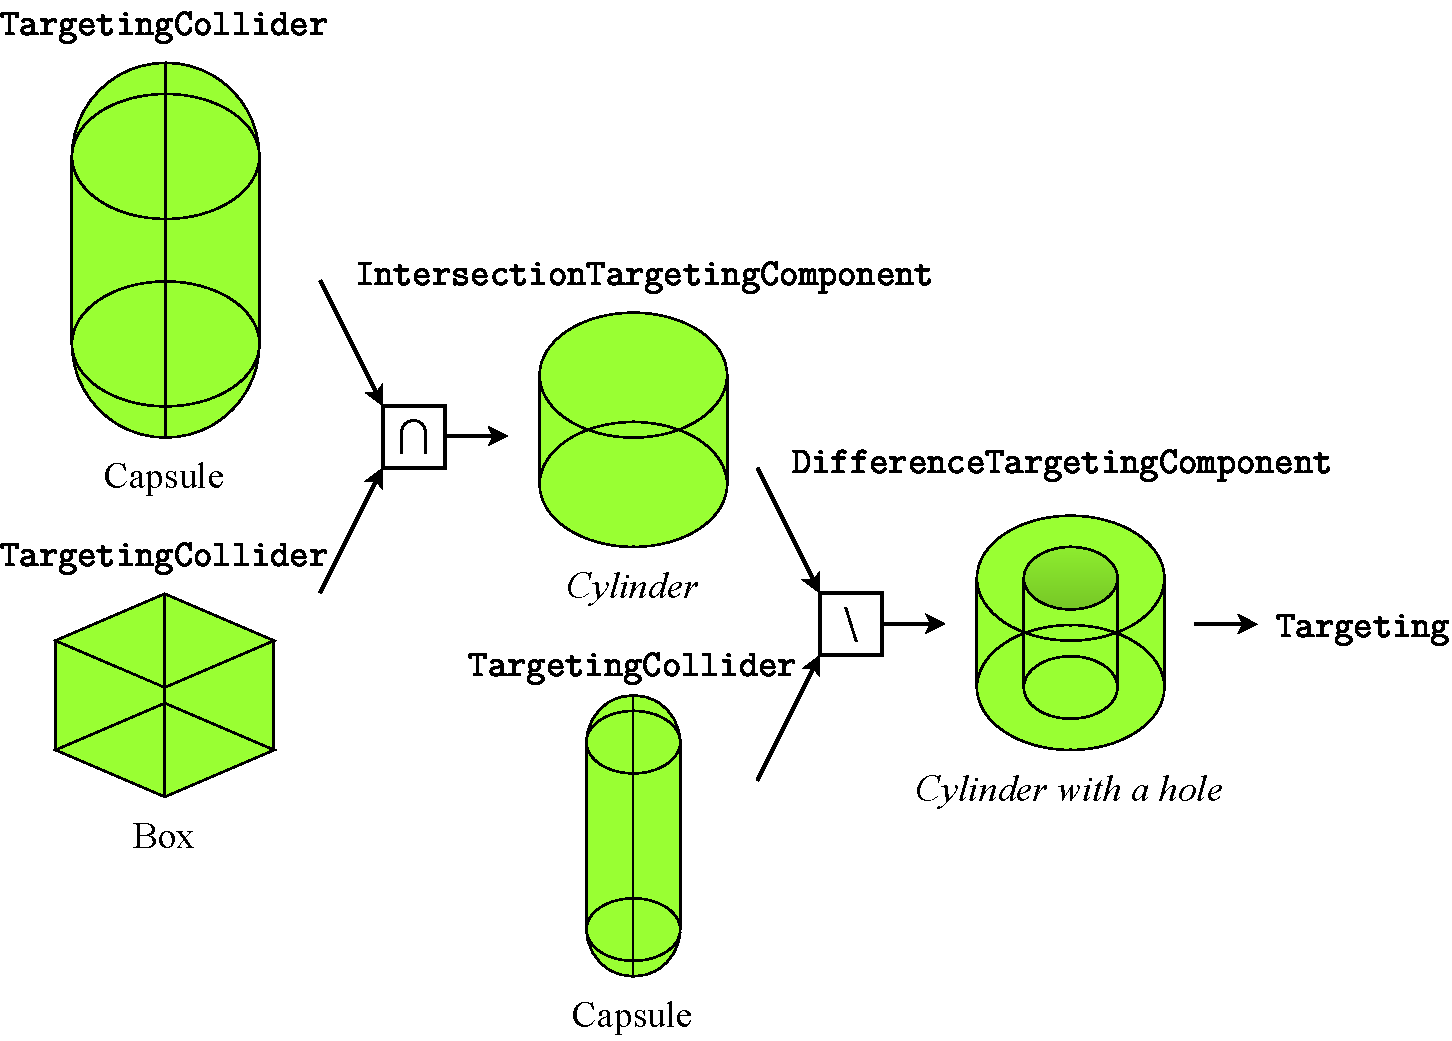
\includegraphics[width=0.8\textwidth]{img/combining colliders.pdf}
    \caption{Combining collider shapes using set operations.}
    \label{fig:combining-colliders}
\end{center}

Most towers ask the \mono{Targeting} every tick they could shoot whether they have a target, and if so, they shoot at it.
Some towers hit their target instantly, but others shoot a projectile, which will take few ticks to hit the target.
Some projectiles might even miss the target.
The behavior of various projectiles is implemented in the derived classes of \mono{Projectile} used in their prefabs.
Once they hit their target, they notify the tower that shot them.

To damage an attacker, the tower should use its method \mono{TryHit}.
The attacker then invokes the \mono{DAMAGE} command, and it also handles this command by decreasing its own HP accordingly.
Similarly, when the player uses an ability to damage attackers, the ability determines its targets, usually using a sphere cast, and damages them via the \mono{TryHit}.
The interactions described in this section are summarized in figure~\ref{fig:shooting}.

\begin{center}
    \captionsetup{type=figure}
    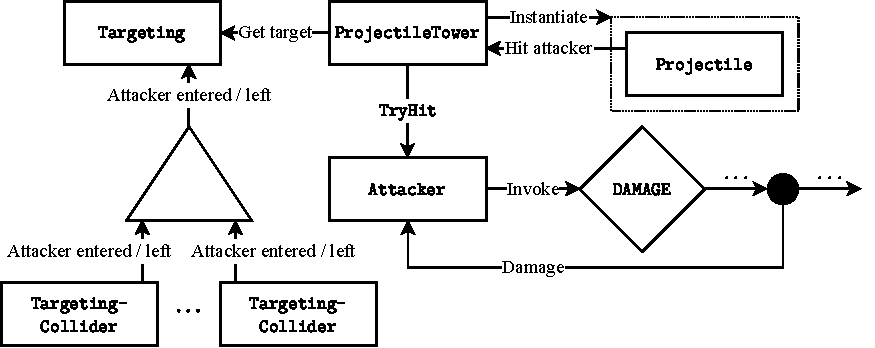
\includegraphics[width=\textwidth]{img/shooting.pdf}
    \caption{Script interactions when a tower shoots at an enemy.}
    \label{fig:shooting}
\end{center}

\subsection{Info Panel}\label{sec:docs-info-panel}

In the following subsections we'll take a look at the more visual elements of the game, whose main job is to communicate information to the player.
We'll start with the info panel.

The info panel exists both in the \emph{Battle} and \emph{Blueprint Selection} scene.
The public methods of its \mono{InfoPanel} script get called directly by various scripts.
To show info about a certain object, the right method is called, and the object is passed as an argument.
The \mono{InfoPanel} saves these references, so it always works with up-to-date information.
The \mono{Hide} method can be used to hide the panel.

To show information about some object, the info panel creates an instance of the corresponding \mono{DescriptionProvider} script.
The \mono{InfoPanel} then asks the \mono{DescriptionProvider} every frame for the current description.
This way, the descriptions can change in real time.
Each \mono{DescriptionProvider} first generates the description with tags as specified in section~\ref{sec:analysis-description-tags}, and then it uses \mono{DescriptionFormatter} to format them into the corresponding formatted text and icons.

Most tags used in the descriptions of buildings or blueprints represent a value that can be modified.
The \mono{Blueprint} script contains a modifiable query for each modifiable value it holds.
The values stored in the blueprint are the base values, and the real up-to-date values are to be obtained through these queries.
For formatting the descriptions, the \mono{DescriptionFormatter} compares these modified values to the base values, and it colors the text based on if the modified value has changed for the better, worse or not at all.

In figure~\ref{fig:description-formatting} we show an example of how a description is produced.
In this case, the info panel is displaying a description of a \emph{Predator} tower, and for that, it has created an instance of a \mono{BlueprintDescriptionProvider}.
In the diagram, the info panel asks the description provider for the description.
The description provider first assembles it from parts provided by the tower and its blueprint, and then it asks the \mono{DescriptionFormatter} to format it.
The \mono{DescriptionFormatter} replaces the tag \enquote{[\$DMG]} with the word \enquote{Damage}, the icon of the damage type, and a colored text with the damage amount.
It reads from the blueprint that in this case, the base damage is 10, and by using the modifiable query \mono{Damage}, it obtains that the current damage should be 17.
So, it outputs that the tower deals 17 damage, and the number is green, because it is greater than the base damage.

\begin{center}
    \captionsetup{type=figure}
    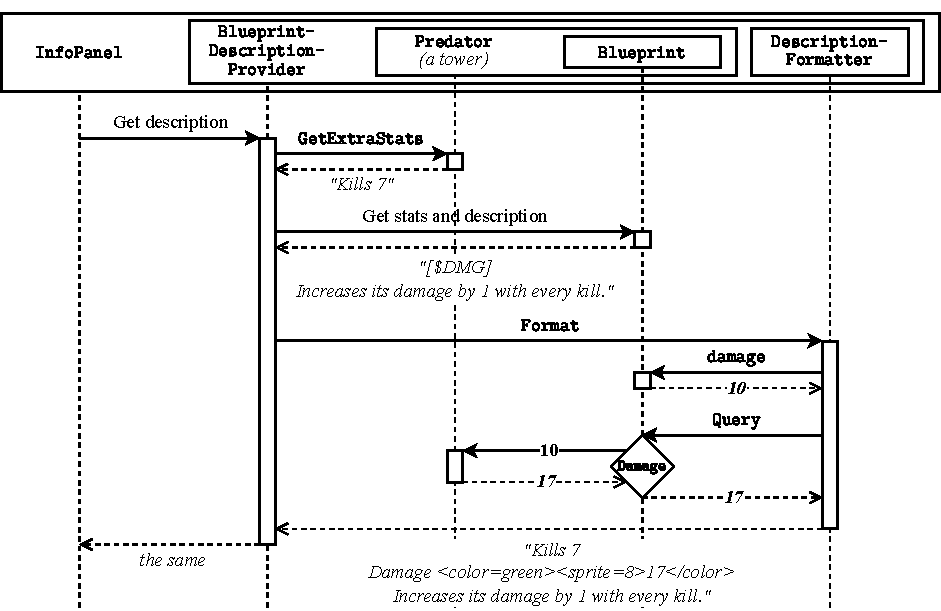
\includegraphics[width=\textwidth]{img/description formatting.pdf}
    \caption{Generating the description to be shown in the info panel.}
    \label{fig:description-formatting}
\end{center}

When a building is selected, the info panel also shows a delete button.
For towers, it also shows arrows that allow the player to change the tower's targeting priority.
Since the info panel has a reference to the building it's displaying information about, it can just directly call the building's public methods for this functionality.
It's important to note that when a building gets destroyed, the building has to unregister all modifiers and reactions it has registered.

\subsection{Visuals and Interpolation}

Scripts that take care of visuals are separated from the game logic.
The visuals scripts have references to the game logic scripts they care about, and they read their public fields, or react to various events.
For example, the scripts that display the player's energy and materials just read the values directly from the \mono{PlayerState} script.
However, sometimes we add some events to the game logic scripts, whose only purpose is to let the visuals know when something happens.
For example, the \mono{SelectionController} has the Unity event \mono{resetVisuals}, which is used to let visuals scripts know that the setup of the blueprint currently being built has changed, so they should reflect this change.

Various visuals scripts also react to the game events.
For example, the \mono{NumberEffects} script spawns a number effect above an attacker whenever the attacker gets damaged, and it creates number effects whenever resources get produced.
These number effects show the amount of damage that was dealt, or the amount and type of the resource produced.

Each blueprinted object also has some scripts that control its visuals.
For example, the script that takes care of the visualization of most projectile-shooting towers is \mono{BasicProjectileTowerVisuals}.
It makes the tower's turret point towards the attacker the tower is targeting, but it also interpolates the rotation to be smooth.
It also subscribes to the tower's \mono{onShoot} Unity event to play an animation when the tower shoots.

We would also like to mention that both attackers and projectiles move the world as a part of the game logic.
Of course, they change their position only 20 times per second, but to the player, their travel needs to look smooth.
So, their visuals scripts simulate their movement in the same way as the game logic scripts, only with a greater temporal resolution.

\subsection{Highlights and Range Visualization}\label{sec:docs-highlights}

When the player selects a building, attacker, or a blueprint, it is highlighted, so the player knows it's selected.
Furthermore, we might highlight other relevant objects differently to show that they are somehow affected by the selected object.
For example, when the player selects a tower, it highlights the attackers in its range in yellow.
We also want to show the affected region of the world, by coloring the terrain accordingly.
For example for towers, we draw their range.
This is described in section~\ref{sec:design-selection-highlights}.

The \mono{HighlightController} looks at the \mono{SelectionController}'s selected and/or hovered objects every frame and determines which objects in the world should be highlighted.
However, each selected object wants to highlight objects differently.
This behavior is implemented in the object's script derived from \mono{HighlightProvider}.
If the selected object has a \mono{HighlightProvider}, or when a selected tile has a building with a \mono{HighlightProvider} on it, the \mono{HighlightController} asks it what objects should be highlighted, and with which color.
It then tells these object to change their highlights accordingly.
The objects that can show highlights implement the interface \mono{IHighlightable}.

The \mono{HighlightController} also closely monitors the \mono{SelectionController} when placing a blueprint.
It highlights the selected tile, or attacker, or it shows just a point highlight which highlights the selected position in the world, based on the blueprinted object's \mono{Placement}.

Each \mono{HighlightProvider} also implements a function that returns the color of the range visualization for any given point, as described in section~\ref{sec:analysis-range}.
The script \mono{RangeVisualization} then creates the range visualization over many frames, based on the \mono{HighlightProvider} that's currently selected according to the \mono{HighlightController}.
The interactions described in this section are shown in figure~\ref{fig:highlights-and-range}.

\begin{center}
    \captionsetup{type=figure}
    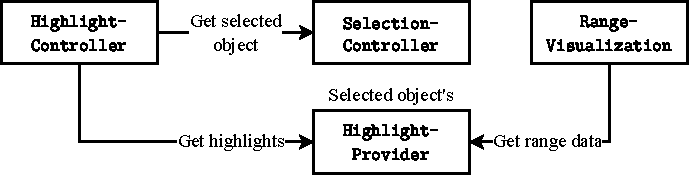
\includegraphics[width=0.9\textwidth]{img/higlights and range.pdf}
    \caption{Interactions between scripts for highlights and range visualization.}
    \label{fig:highlights-and-range}
\end{center}

In addition to our specification in section~\ref{sec:analysis-range}, when placing a blueprint, the \mono{HighlightProvider} also shows in blue the valid positions to place it.
For this, it needs a reference to the given \mono{Placement} script to ask it which positions are valid.

\subsection{Tutorial}

The tutorial is handled by a system separate from other scripts.
It calls their public methods, and modifies their data to achieve the behavior we want.
There are two scripts that handle the tutorial:

\mono{TutorialController} keeps track of the player's progress through the tutorial.
The tutorial is a sequence of steps, and the \mono{TutorialController} has a Unity event for each of them.
At the start of each step, it invokes the corresponding Unity event.
This way, all things that happen during the tutorial can be assigned in the Unity editor.

The script \mono{TutorialActions} then contains methods which do various modifications to various objects within the scene, so these actions can be subscribed to the \mono{TutorialController} Unity events.
\mono{TutorialActions} also contains various checks based on which it tells the \mono{TutorialController} when to go to the next step.

\section{Game Start and Procedural Generation}\label{sec:docs-data}

In this section we'll take a look at the processes that happen from the application start, all the way to generating worlds and waves.
We already described the transitions between scenes in section~\ref{sec:docs-scenes}, and now we'll go into more detail.

\subsection{Loading}

When the application starts, a \enquote{Made with Unity} splash screen is shown, and then the \emph{Loading} scene is loaded.
As we mentioned in section~\ref{sec:docs-scripts}, this scene contains \mono{SceneController} and \mono{SoundController}~--- game objects that persist throughout the entirety of the application runtime and provide useful functionality.
However, the main purpose of this scene is to load various data from the disk into memory.
This is handled by the \mono{StartLoader} script.
We can register to it any number of \mono{ILoader} scripts, which do the loading and store the data in singleton classes.

Currently, the only loader we use is \mono{TerrainTypeLoader}, which loads the terrain types from the \emph{StreamingAssets/TerrainTypes} folder.
For each terrain type file, the \mono{TerrainTypeLoader} creates a new \mono{TerrainType} object using the function \mono{Parse} it has.
The parsing is done using a simple parser implemented in the folder \emph{Scripts/Data/Parsers}.
The terrain type file format is described in section~\ref{sec:docs-terrain-type}.

\subsection{Menus and Starting a Run}

The \emph{Menu} scene contains mostly just three buttons and an object with the \mono{RunStarter} script.
All three buttons call a method on the \mono{RunStarter} when pressed.
When the \enquote{Start} button is pressed, the \mono{RunStarter} instantiates the \emph{RunPersistence} prefab, configures it, and calls the \mono{NextLevel()} method on its \mono{RunPersistence} script.

Pressing the \enquote{Custom Run} button takes the player to the \emph{Run Settings} scene.
It contains more UI elements, and another object with a \mono{RunStarter} script.
Here, the player can change the run settings by interacting with the UI elements, which in turn notify the \mono{RunStarter} about these changes.
When the player starts the run, the instantiated \emph{RunPersistence} prefab is then configured according to the settings.
If the \enquote{Select starting blueprints} option is enabled, instead of going to the first level, the scene \emph{Blueprint Selection} is loaded, where the player can select the starting blueprints.

\subsection{Run Persistence and Blueprint Rewards}\label{sec:docs-run-persistence}

The \emph{RunPersistence} object persists between scenes, and it only destroys itself when a run ends.
It holds all scripts that need to remember some state throughout the whole run:
The \mono{RunPersistence} script keeps track of the player's hull and blueprints, the run seed, the current level, and it gives orders to the other scripts.
The \mono{BlueprintRewardController} script generates blueprint rewards for the player.

After the player beats a level, the \mono{RunPersistence} asks the \mono{BlueprintRewardController} to reward the player with blueprints.
For the rewards after the first tutorial level, the \mono{BlueprintRewardController} has a predefined blueprint selection, but for normal blueprint rewards, it picks the selection randomly, based on its seed.
It then changes the scene to the \emph{Blueprint Selection} scene, and initializes the \mono{BlueprintSelectionController} script in it with the selection.

The \mono{BlueprintSelectionController} handles the blueprint selection.
It initializes the scene by instantiating \emph{BlueprintDisplay} prefabs which depict the blueprints on offer and the player's current collection.
When the player clicks on one of the blueprints, it notifies the \mono{BlueprintSelectionController}, which handles the selection logic.
It also modifies the blueprints' outlines to communicate to the player what is selectable or selected, and it makes the info panel show relevant information.
Once the player confirms their selection by clicking on a button, it returns what the player chose in a callback to the \mono{RunPersistence}, which updates the player's blueprint collection and proceeds to the next level.

The interactions described in this section are summarized in figure~\ref{fig:blueprint-selection}.
\begin{center}
    \captionsetup{type=figure}
    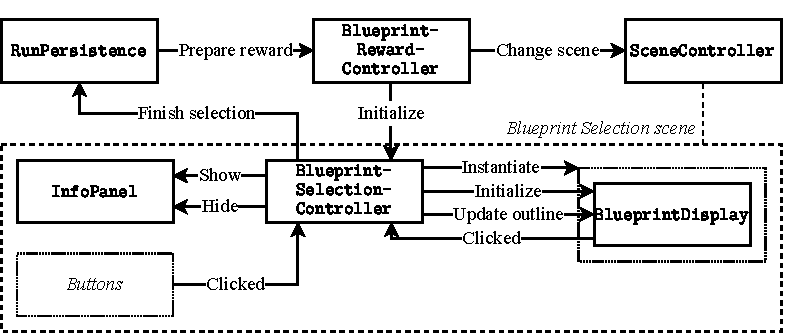
\includegraphics[width=\textwidth]{img/blueprint selection.pdf}
    \caption{Interactions between scripts during blueprint selection.}
    \label{fig:blueprint-selection}
\end{center}

\subsection{Seed Branching and Level Initialization}\label{sec:docs-level-init}

As we described in section~\ref{sec:analysis-rng}, we use \emph{seed branching} everywhere throughout the procedural generation.
This means that whenever some system needs RNG, it gets a seed from another system, and from this seed it creates its own RNG instance to use.
Figure~\ref{fig:seed-branching} shows how the seeds get propagated across the game's systems.
When starting a new run, the \mono{RunStarter} creates a new instance of \mono{RunPersistence}, and it is given a run seed.
It is either randomly generated using \mono{System.Random} or selected by the player.
The \mono{RunPersistence} then initializes the \mono{BlueprintRewardController}, giving it a seed to generate rewards from.

Whenever a new level is started, the \mono{WorldGenerator} in the \emph{Battle} scene finds the \mono{RunPersistence} and asks it to set up the level settings.
For this, the \mono{RunPersistence} uses the \mono{LevelSetter} script, which finds the relevant scripts in the scene and sets them up.
The \mono{RunPersistence} generates a seed for the \mono{LevelSetter}.
The \mono{LevelSetter} generates a new seed for the world generator and configures the number of paths and their lengths, based on the level number, storing this information in the \mono{WorldSettings} script.
It also configures the \mono{WaveGenerator}'s seed and parameters, and the fuel goal in the \mono{PlayerState}.
Figure~\ref{fig:seed-branching} shows the \mono{WorldSettings} and \mono{WaveGenerator} multiple times, to convey that each level has a new instance of these scripts.

\begin{center}
    \captionsetup{type=figure}
    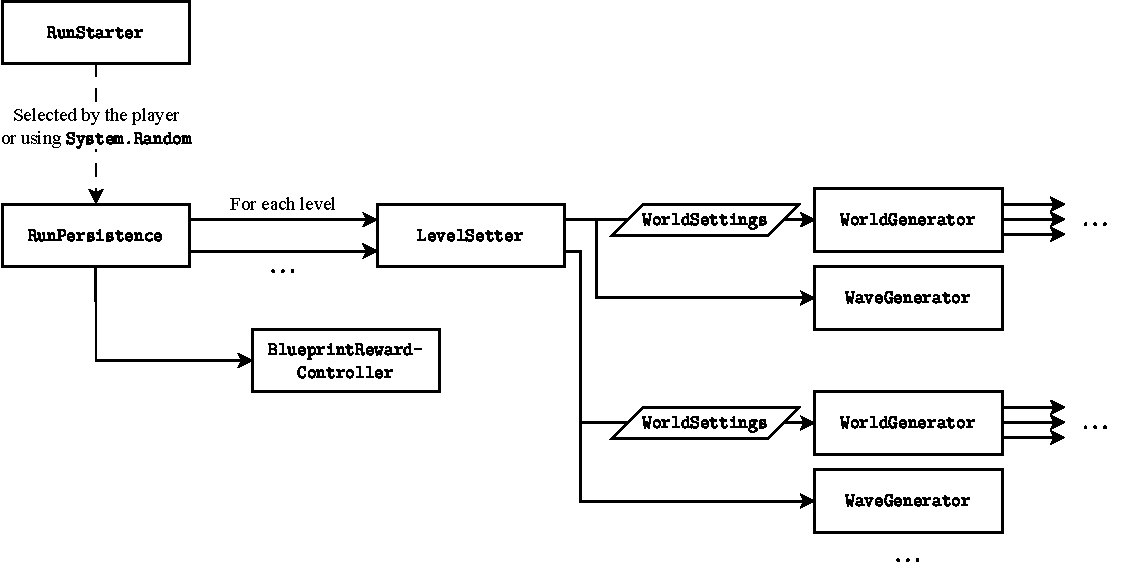
\includegraphics[width=\textwidth]{img/seed splitting.pdf}
    \caption{Seed propagation using seed branching.}
    \label{fig:seed-branching}
\end{center}

\subsection{Procedural World Generation}\label{sec:docs-world-generation}

The \mono{WorldGenerator} handles the world generation by giving orders to other scripts.
We illustrate its interactions with other scripts in figure~\ref{fig:world-generator}.
As we mentioned, when the \emph{Battle} scene is loaded, it asks the \mono{RunPersistence} to set up the level.
All information the \mono{WorldGenerator} needs is supplied through the \mono{WorldSettings} script.
The world generator then reads the information, and calls other generator scripts, which each take care of one stage of the world generation, as described in section~\ref{sec:analysis-procedural-generation}.

\begin{center}
    \captionsetup{type=figure}
    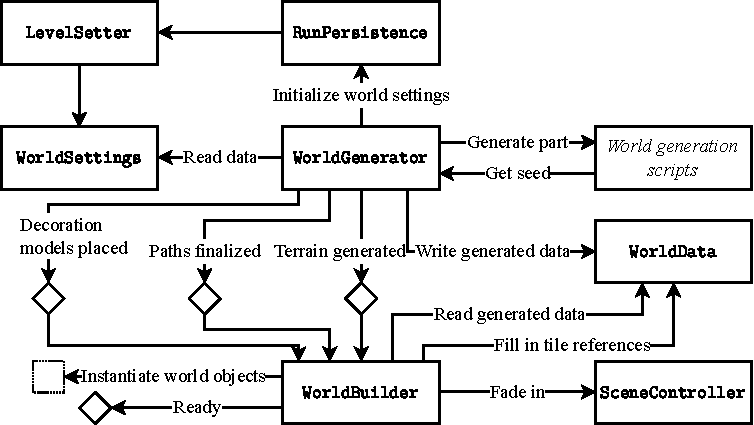
\includegraphics[width=\textwidth]{img/world generator.pdf}
    \caption{Script interactions during world generation.}
    \label{fig:world-generator}
\end{center}

In order of use, the world generation scripts are:
\begin{enumerate}
    \item \mono{PathEndPointPicker} picks path end points (section~\ref{sec:analysis-path-starts}).
    \item \mono{PathPlanner} generates main paths (section~\ref{sec:analysis-main-paths}).
    \item \mono{WFCGenerator} generates the terrain (section~\ref{sec:analysis-terrain-generation}).
    \item \mono{ObstacleGenerator} selects the positions for obstacles (section~\ref{sec:analysis-obstacles}).
    \item \mono{PathFinalizer} then creates the final path network (section~\ref{sec:analysis-final-paths}).
    \item \mono{ObstacleModelScatterer} selects the obstacle model positions and sizes (section~\ref{sec:analysis-obstacles}).
\end{enumerate}

The \mono{WorldGenerator} gives each script the information it needs, be it from the \mono{WorldSettings} or data that was generated in some previous stage.
All the algorithms are randomized, and they can require multiple random number generators.
To generate seeds for their RNG's, they use the \mono{WorldGenerator}'s RNG that was initialized with the seed from \mono{WorldSettings}.
After each stage, the \mono{WorldGenerator} writes the generated data into the \mono{WorldData} script.
From the \mono{WorldData}, other scripts can read the information about the generated world, as also mentioned in section~\ref{sec:docs-battle-scene}.
After several stages, the \mono{WorldGenerator} invokes an event to notify other scripts that new world data is ready.

The world generation stages done in background threads so that the game doesn't become unresponsive.
however, in Unity, we cannot instantiate objects from a background thread.
The script \mono{WorldBuilder} reacts to the \mono{WorldGenerator}'s events, and it builds the terrain, obstacles, paths, and tiles in the main thread.
It also reads the world data from the \mono{WorldData} script, and writes back references to the tile instances it created.

Creating many objects is expensive, so to prevent stuttering, we use Unity coroutines to build the world across multiple frames.
Currently, the screen is faded out using the \mono{SceneController} during world generation, but later we'd like to add an animation, which would make any stutters obvious.
Once the \mono{WorldBuilder} finishes building the world, it tells the \mono{SceneController} to fade in the screen, and it invokes an event to notify all other scripts that the world is generated.
\chapter{User Documentation --- Designer}

In this chapter, we'll describe how one might go about adding new content to the game.
We'll describe how to add new Attackers, Blueprints and Terrain types, each in its own section.
For all these content types, we recommend taking inspiration from the content already in the game, or even creating a copy and editing it as needed.

\section{Attackers}

To add a new attacker, we start by creating new \mono{AttackerStats} scriptable object.
These are stored in the \emph{AttackerStats} assets folder.
To create new \mono{AttackerStats} scriptable object, in Unity, right-click in the folder and select \emph{Create > AttackerStats}.
For this attacker to appear in the game, we must assign it to the wave generator's selection.
To do this, open the scene \emph{Scenes/Battle}.
In it, find the game object \emph{World > WaveGenerator} and add the new \mono{AttackerStats} to the \emph{Available Attackers} array of its \mono{WaveGenerator} script.



- assign to the wave generator

\section{Blueprints}

\section{Terrain Types}
\chapter{User Documentation}\label{user-docs}

The demo version of our game is called \enquote{Project Nitrogen}, and it is available in the attachments as the folder \emph{Build}.
This is a build for a personal computer with the \emph{Windows} operating system.
In this chapter, we will give instructions on how to run the game, how to navigate its menus, and we provide some reference tables with information the player might find useful.

\section{Instructions}

The attachment folder \emph{Build} contains a few application binaries, a dynamically linked library and directories with the game's assets.
To run the game, simply run the \mono{ProjectNitrogen.exe} binary.

The game will show a \enquote{Made with Unity} splash screen and take you to the main menu.
The main menu contains three large buttons: \enquote{Start}, \enquote{Custom Run} and  \enquote{Exit}.
To start a new run, click the \enquote{Start} button.
The \enquote{Custom Run} button will take you to the run settings screen, and the \enquote{Exit} button will exit the game.

The run settings screen lets you set the seed of the run, and it lets you choose to select the starting blueprints at the start of the run.
To start the run with these settings, press the \enquote{Start} button.
The \enquote{Replay Tutorial} button will disregard these settings, and start a tutorial run instead.
To return to the main menu, press the \enquote{Back} button.

The first run started from the main menu will include the in-game tutorial, which explains how to play the game in an interactive manner.
It explains the goals of the game and the game's controls.

\section{Reference Tables}

In this section, we provide some tables the players might find useful.
The in-game tutorial explains how to control the game, but table~\ref{tab:controls} contains all controls and hotkeys the player can use during battle for reference.
Some hotkeys are not mentioned in the game, but they are not necessary to play it.

We also provide reference tables with all the attackers and blueprints the game contains.
Attackers are in tables~\ref{tab:attackers1} and~\ref{tab:attackers2}.
Blueprints are separated by type:
\begin{itemize}
    \item Economic buildings~--- table~\ref{tab:economic-buildings}.
    \item Special buildings~--- table~\ref{tab:special-buildings}.
    \item Tower~--- tables~\ref{tab:towers1} and~\ref{tab:towers2}.
    \item Abilities~--- table~\ref{tab:abilities}.
\end{itemize}

\begin{table}[H]
    \centering
    \begin{tabular}{m{0.2\textwidth}m{0.7\textwidth}}
        \toprule
        \textbf{Button}                                   & \textbf{Actions}                                                     \\
        \midrule
        \textbf{Left click}                               & Press a user interface button. \vspace{4pt}\newline
        Select a tile, building or attacker in the world, or a blueprint from the blueprint menu. \vspace{4pt}\newline
        Deselect currently selected object (except for a blueprint) and hide the info panel by clicking on empty space.          \\\midrule
        \textbf{Right click}                              & Deselect currently selected object and hide the info panel.          \\\midrule
        \textbf{Right click \newline drag}                & Move the camera.                                                     \\\midrule
        \textbf{Scrolling}                                & Zoom the camera in or out.                                           \\\midrule
        \textbf{Scroll wheel \newline drag}               & Rotate the camera to the left or right.                              \\\midrule
        \textbf{Escape}                                   & Deselect currently selected object and hide the info panel.          \\\midrule
        \textbf{Space}                                    & Start the next wave.                                                 \\\midrule
        \textbf{1} to \textbf{9}                          & Select the 1st to 9th blueprint from the blueprint menu.             \\\midrule
        \textbf{R}                                        & Rotate the currently selected blueprint, if possible.                \\\midrule
        \textbf{W} / \textbf{S} / \textbf{A} / \textbf{D} & Move the camera forward / back / left / right.                       \\\midrule
        \textbf{T} / \textbf{G}                           & Zoom the camera in / out.                                            \\\midrule
        \textbf{Q} / \textbf{E}                           & Rotate the camera left / right.                                      \\\midrule
        \textbf{Tab}                                      & Change the targeting priority of the selected tower to the next.     \\\midrule
        \textbf{Ctrl} + \textbf{Tab}                      & Change the targeting priority of the selected tower to the previous. \\\midrule
        \textbf{Delete}                                   & Delete the selected building.                                        \\\midrule
        \textbf{M}                                        & Mute or unmute the game sounds.                                      \\
        \bottomrule
    \end{tabular}
    \caption{The controls and hotkeys the player can use during a battle.}
    \label{tab:controls}
\end{table}


\begin{table}[H]
    \centering
    \begin{tabular}{m{9mm}m{25mm}D{.}{.}{-1}rm{0.48\textwidth}}
        \toprule
        \textbf{Icon}                                                                 & \textbf{Name}                          & \mc{\textbf{Speed}} & \mc{\textbf{HP}} & \textbf{Description}                                                                                                                                \\
        \midrule
        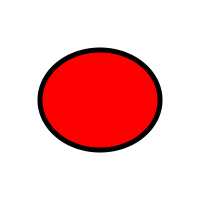
\includegraphics[height=7mm]{img/Icons/Attackers/Red Slime.png}               & \footnotesize{Red Slime}               & 1                   & 5                &                                                                                                                                                     \\
        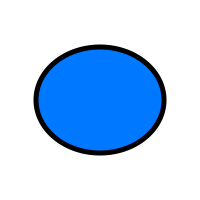
\includegraphics[height=7mm]{img/Icons/Attackers/Blue Slime.png}              & \footnotesize{Blue Slime}              & 1.4                 & 10               & \footnotesize{When killed, spawns a \emph{Red Slime}.}                                                                                              \\
        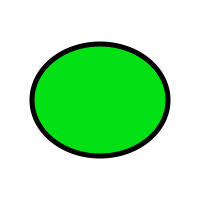
\includegraphics[height=7mm]{img/Icons/Attackers/Green Slime.png}             & \footnotesize{Green Slime}             & 1.8                 & 15               & \footnotesize{When killed, spawns a \emph{Blue Slime}.}                                                                                             \\
        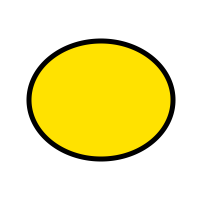
\includegraphics[height=7mm]{img/Icons/Attackers/Yellow Slime.png}            & \footnotesize{Yellow Slime}            & 3.2                 & 20               & \footnotesize{When killed, spawns a \emph{Green Slime}.}                                                                                            \\
        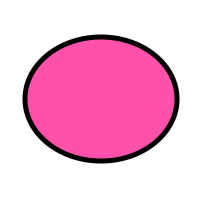
\includegraphics[height=7mm]{img/Icons/Attackers/Pink Slime.png}              & \footnotesize{Pink Slime}              & 3.5                 & 25               & \footnotesize{When killed, spawns a \emph{Yellow Slime}.}                                                                                           \\
        
\includegraphics[height=7mm]{img/Icons/Attackers/Black Slime.png}             & \footnotesize{Black Slime}             & 1.8                 & 30               & \footnotesize{Immune to \emph{Explosive} damage. \newline When killed, spawns two \emph{Pink Slimes}.}                                              \\
        
\includegraphics[height=7mm]{img/Icons/Attackers/Lead Slime.png}              & \footnotesize{Lead Slime}              & 1                   & 35               & \footnotesize{Immune to \emph{Physical} damage. \newline When killed, spawns two \emph{Black Slimes}.}                                              \\
        
\includegraphics[height=7mm]{img/Icons/Attackers/Skeleton.png}                & \footnotesize{Skeleton}                & 1.6                 & 20               &                                                                                                                                                     \\
        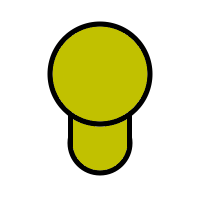
\includegraphics[height=7mm]{img/Icons/Attackers/Yellow Skeleton.png}         & \footnotesize{Yellow Skeleton}         & 1.6                 & 60               &                                                                                                                                                     \\
        
\includegraphics[height=7mm]{img/Icons/Attackers/Black Skeleton.png}          & \footnotesize{Black Skeleton}          & 1.6                 & 180              &                                                                                                                                                     \\
        
\includegraphics[height=7mm]{img/Icons/Attackers/Armored Skeleton.png}        & \footnotesize{Armored Skeleton}        & 0.8                 & 40               & \footnotesize{Has shields that block 1 damage from each hit. \newline Once HP drops below half of max HP, loses the shields and doubles its speed.} \\
        
\includegraphics[height=7mm]{img/Icons/Attackers/Armored Yellow Skeleton.png} & \footnotesize{Yellow Armored Skeleton} & 0.8                 & 120              & \footnotesize{Has shields that block 3 damage from each hit. \newline Once HP drops below half of max HP, loses the shields and doubles its speed.} \\
        
\includegraphics[height=7mm]{img/Icons/Attackers/Armored Black Skeleton.png}  & \footnotesize{Black Armored Skeleton}  & 0.8                 & 360              & \footnotesize{Has shields that block 5 damage from each hit. \newline Once HP drops below half of max HP, loses the shields and doubles its speed.} \\
        
\includegraphics[height=7mm]{img/Icons/Attackers/Big Skull.png}               & \footnotesize{Big Skull}               & 1.2                 & 10               & \footnotesize{\textbf{Large.} \newline When killed, spawns 3 \emph{Skeletons}.}                                                                     \\
        
\includegraphics[height=7mm]{img/Icons/Attackers/Big Yellow Skull.png}        & \footnotesize{Big Yellow Skull}        & 1.2                 & 30               & \footnotesize{\textbf{Large.} \newline When killed, spawns 3 \emph{Yellow Skeletons}.}                                                              \\
        
\includegraphics[height=7mm]{img/Icons/Attackers/Big Black Skull.png}         & \footnotesize{Big black Skull}         & 1.2                 & 90               & \footnotesize{\textbf{Large.} \newline When killed, spawns 3 \emph{Black Skeletons}.}                                                               \\
        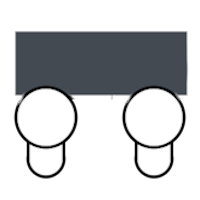
\includegraphics[height=7mm]{img/Icons/Attackers/Coffin.png}                  & \footnotesize{Coffin}                  & 0.4                 & 80               & \footnotesize{\textbf{Large.} \newline Spawns an \emph{Armored Skeleton} every 4s. \newline When killed, spawns 4 \emph{Skeletons}.}                \\
        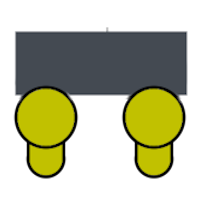
\includegraphics[height=7mm]{img/Icons/Attackers/Yellow Coffin.png}           & \footnotesize{Yellow Coffin}           & 0.4                 & 240              & \footnotesize{\textbf{Large.} \newline Spawns a \emph{Yellow Armored Skeleton} every 5s. \newline When killed, spawns 4 \emph{Yellow Skeletons}.}   \\
        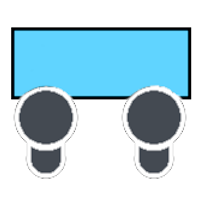
\includegraphics[height=7mm]{img/Icons/Attackers/Black Coffin.png}            & \footnotesize{Black Coffin}            & 0.4                 & 720              & \footnotesize{\textbf{Large.} \newline Spawns a \emph{Black Armored Skeleton} every 6s. \newline When killed, spawns 4 \emph{Black Skeletons}.}     \\
        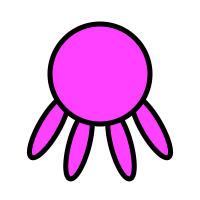
\includegraphics[height=7mm]{img/Icons/Attackers/Jellyfish.png}               & \footnotesize{Space Jellyfish}         & 0.8                 & 8                & \footnotesize{Takes 40\% less \emph{Physical} damage.}                                                                                              \\
        
\includegraphics[height=7mm]{img/Icons/Attackers/Blue Jellyfish.png}          & \footnotesize{Blue Space Jellyfish}    & 0.8                 & 40               & \footnotesize{Takes 50\% less \emph{Physical} damage.}                                                                                              \\
        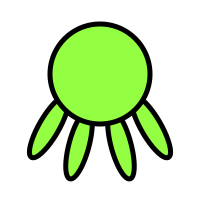
\includegraphics[height=7mm]{img/Icons/Attackers/Green Jellyfish.png}         & \footnotesize{Green Space Jellyfish}   & 0.8                 & 200              & \footnotesize{Takes 66\% less \emph{Physical} damage.}                                                                                              \\
        \bottomrule
    \end{tabular}
    \caption{The attacker types in the game (part 1).}
    \label{tab:attackers1}
\end{table}

\begin{table}[H]
    \centering
    \begin{tabular}{m{9mm}m{25mm}D{.}{.}{-1}rm{0.48\textwidth}}
        \toprule
        \textbf{Icon}                                                       & \textbf{Name}                & \mc{\textbf{Speed}} & \mc{\textbf{HP}} & \textbf{Description}                                                                                                                                        \\
        \midrule
        
\includegraphics[height=7mm]{img/Icons/Attackers/Fire Spirit.png}   & \footnotesize{Fire Spirit}   & 3                   & 6                & \footnotesize{Takes 50\% less \emph{Energy} damage.}                                                                                                        \\
        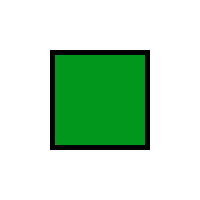
\includegraphics[height=7mm]{img/Icons/Attackers/Forest Spirit.png} & \footnotesize{Forest Spirit} & 2                   & 15               & \footnotesize{Takes 66\% less \emph{Explosive} damage.}                                                                                                     \\
        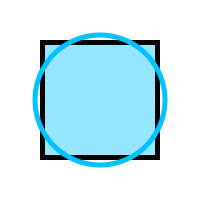
\includegraphics[height=7mm]{img/Icons/Attackers/Protector.png}     & \footnotesize{Protector}     & 1.4                 & 100              & \footnotesize{\textbf{Large.} \newline When killed, leaves behind a protective bubble 1.3 tiles in radius that blocks all projectiles from outside for 5s.} \\
        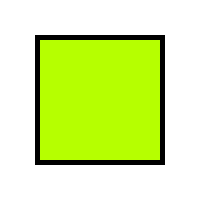
\includegraphics[height=7mm]{img/Icons/Attackers/Druid.png}         & \footnotesize{Druid}         & 1                   & 120              & \footnotesize{\textbf{Large.} \newline Every 4s heals each attacker in a 1.6 tile radius by 15 HP.}                                                         \\
        \bottomrule
    \end{tabular}
    \caption{The attacker types in the game (part 2).}
    \label{tab:attackers2}
\end{table}


\begin{table}[H]
    \centering
    \begin{tabular}{m{15mm}m{20mm}lm{0.5\textwidth}}
        \toprule
        \textbf{Icon}                                                            & \textbf{Name}           & \textbf{Rarity} & \textbf{Description}                                                                             \\
        \midrule
        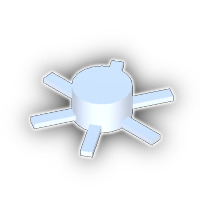
\includegraphics[height=15mm]{img/Icons/Buildings/Dust Collector.png}    & Dust \newline Refinery  & Common          &
        \footnotesize{\textbf{Cost: 5 materials} \newline Produces 5 materials after every wave. \newline Cannot be placed on slants and adjacent to another Dust Refinery. \newline Increases cost by 5 materials when built.} \\

        \includegraphics[height=15mm]{img/Icons/Buildings/Energy Harvester.png}  & Energy Harvester        & Rare            &
        \footnotesize{\textbf{Cost: 15 materials} \newline Whenever you gain Materials, produces 40\% as much Energy.}                                                                                                          \\

        \includegraphics[height=15mm]{img/Icons/Buildings/Fuel Refinery.png}     & Fuel \newline Extractor & Rare            &
        \footnotesize{\textbf{Cost: 30 materials} \newline Cooldown 1 \newline Must be built on tiles rich in fuel. \newline Produces 10 fuel after every wave.}                                                                \\

        \includegraphics[height=15mm]{img/Icons/Buildings/Matter Replicator.png} & Matter Replicator       & Rare            &
        \footnotesize{\textbf{Cost: 30 materials} \newline Cooldown 2 \newline Produces 5 materials after every wave, then increases its production by 5 materials.}                                                            \\

        \includegraphics[height=15mm]{img/Icons/Buildings/Solar Panel.png}       & Solar Panel             & Common          &
        \footnotesize{\textbf{Cost: 5 materials} \newline Cannot be paced on slanted tiles. \newline The higher it's placed, the more energy it produces after every wave: 2 for every level of height.}                        \\

        \includegraphics[height=15mm]{img/Icons/Buildings/Surface Drill.png}     & Surface Drill           & Starter         &
        \footnotesize{\textbf{Cost: 10 materials} \newline Must be built on tiles rich in minerals or fuel. \newline Produces 5 materials or 2 fuel after every wave.}                                                          \\
        \bottomrule
    \end{tabular}
    \caption{The economic building blueprints in the game.}
    \label{tab:economic-buildings}
\end{table}


\begin{table}[H]
    \centering
    \begin{tabular}{m{15mm}m{20mm}lm{0.5\textwidth}}
        \toprule
        \textbf{Icon}                                                          & \textbf{Name}      & \textbf{Rarity} & \textbf{Description}                                               \\
        \midrule
        \includegraphics[height=15mm]{img/Icons/Buildings/Amplifier.png}       & Amplifier          & Legendary       &
        \footnotesize{\textbf{Cost: 40 materials} \newline Cooldown 2 \newline Range 2.3 \newline Increases damage of all towers in range by 3.}                                           \\

        \includegraphics[height=15mm]{img/Icons/Towers/Frostbite Frontier.png} & Frostbite Frontier & Legendary       &
        \footnotesize{\textbf{Cost: 25 materials} \newline Range 2.1 \newline Freezes attackers in range, making them move 25\% slower and take 50\% more Energy damage.}                  \\

        \includegraphics[height=15mm]{img/Icons/Buildings/Hub.png}             & Hub                & Special         &
        \footnotesize{Produces 10 fuel, 10 materials and 10 energy after every wave. \newline When an enemy reaches this building, you lose Hull, up to 5 per wave. Protect at all costs!} \\

        \includegraphics[height=15mm]{img/Icons/Buildings/Radar.png}           & Radar              & Rare            &
        \footnotesize{\textbf{Cost: 10 materials} \newline Increases the range of adjacent buildings by 30\%.}                                                                             \\
        \bottomrule
    \end{tabular}
    \caption{The special building blueprints in the game.}
    \label{tab:special-buildings}
\end{table}


\begin{table}[H]
    \centering
    \begin{tabular}{m{15mm}m{20mm}lm{0.5\textwidth}}
        \toprule
        \textbf{Icon}                                                     & \textbf{Name} & \textbf{Rarity} & \textbf{Description}                                                                                                                                                                                                              \\
        \midrule
        \includegraphics[height=15mm]{img/Icons/Towers/Budget Sentry.png} & Budget Sentry & Starter         &
        \footnotesize{\textbf{Cost: 10 materials} \newline Range 2.9 \newline Damage 2 (physical) \newline Interval 0.8s \newline Shoots projectiles at attackers in line of sight.}                                                                                                                                                            \\

        \includegraphics[height=15mm]{img/Icons/Towers/Double Sentry.png} & Double Sentry & Common          &
        \footnotesize{\textbf{Cost: 15 materials} \newline Range 2.4 \newline Damage 2 (physical) \newline Interval 0.4s \newline Shoots projectiles at attackers in line of sight.}                                                                                                                                                            \\

        \includegraphics[height=15mm]{img/Icons/Towers/Galvanizer.png}    & Galvanizer    & Rare            &
        \footnotesize{\textbf{Cost: 10 energy 40 materials} \newline Range 3.7 \newline Damage 5 (physical) \newline Interval 0.5s \newline Shoots projectiles at attackers in line of sight. \newline When idle for 1.8s, charges up the next shot, making it deal additional 10 Energy damage and produce 5 energy when it hits an attacker.} \\

        \includegraphics[height=15mm]{img/Icons/Towers/Gatling Gun.png}   & Gatling Gun   & Common          &
        \footnotesize{\textbf{Cost: 40 materials} \newline Range 3.3 \newline Damage 2 (physical) \newline Interval 0.15s \newline Needs to shoot continuously for 5s to spin up to maximum fire rate.}                                                                                                                                         \\
        \bottomrule
    \end{tabular}
    \caption{The tower blueprints in the game (part 1).}
    \label{tab:towers1}
\end{table}


\begin{table}[H]
    \centering
    \begin{tabular}{m{15mm}m{20mm}lm{0.5\textwidth}}
        \toprule
        \textbf{Icon}                                                      & \textbf{Name}  & \textbf{Rarity} & \textbf{Description}                                                                                                                                                                            \\
        \midrule
        \includegraphics[height=15mm]{img/Icons/Towers/Mortar.png}         & Mortar         & Starter         &
        \footnotesize{\textbf{Cost: 25 materials} \newline Range 3.7 \newline Damage 4 (explosive) \newline Interval 2s \newline Cannot be paced on slanted tiles. \newline Shoots a cannonball over obstacles, impacting the ground after 1s and dealing damage to attackers within 1.2 tiles.}                \\

        \includegraphics[height=15mm]{img/Icons/Towers/Predator.png}       & Predator       & Legendary       &
        \footnotesize{\textbf{Cost: 50 materials} \newline Range 3.4 \newline Damage 10 (physical) \newline Interval 1s \newline Shoots projectiles at attackers in line of sight. \newline Increases its damage by 1 with every kill.}                                                                         \\

        \includegraphics[height=15mm]{img/Icons/Towers/Sledgehammer.png}   & Sledge-hammer  & Common          &
        \footnotesize{\textbf{Cost: 45 materials} \newline Range 1.6 \newline Damage 20 (explosive) \newline Interval 2.5s \newline Cannot be paced on slanted tiles. \newline Can be placed on tiles with small obstacles. \newline Smashes into the ground, dealing damage to all attackers in range.}        \\

        \includegraphics[height=15mm]{img/Icons/Towers/Sniper.png}         & Sniper         & Common          &
        \footnotesize{\textbf{Cost: 20 materials} \newline Range 11.1 \newline Damage 10 (physical) \newline Interval 3.3s \newline Shoots projectiles at attackers in line of sight. \newline The further away an attacker is, the more damage it takes, up to 200\%.}                                         \\

        \includegraphics[height=15mm]{img/Icons/Towers/Static Sparker.png} & Static Sparker & Common          &
        \footnotesize{\textbf{Cost: 15 materials} \newline Range 3.3 \newline Damage 4 (energy) \newline Interval 1.9s \newline Hits its target, and then up to 3 more within 1.8 tiles from it, dealing half damage to each of them.}                                                                          \\

        \includegraphics[height=15mm]{img/Icons/Towers/Ultra-Ray.png}      & Ultra-Ray      & Rare            &
        \footnotesize{\textbf{Cost: 30 materials} \newline Range 8.1 \newline Damage 1 (energy) \newline Interval 0.15s \newline Press [R] to rotate. \newline Can be placed on tiles with small obstacles. \newline Fires a continuous beam in a fixed cardinal direction, hitting up to 5 attackers at once.} \\
        \bottomrule
    \end{tabular}
    \caption{The tower blueprints in the game (part 2).}
    \label{tab:towers2}
\end{table}


\begin{table}[H]
    \centering
    \begin{tabular}{m{15mm}m{20mm}lm{0.5\textwidth}}
        \toprule
        \textbf{Icon}                                                          & \textbf{Name}   & \textbf{Rarity} & \textbf{Description}                                                                                                                                                                                                                                                  \\
        \midrule
        \includegraphics[height=15mm]{img/Icons/Abilities/Catalyst.png}        & Catalyst        & Rare            &
        \footnotesize{\textbf{Cost: 20 energy} \newline Cooldown 1 \newline Radius 0.8 \newline Afflicts attackers within radius, making them take 2x as much damage and produce 1 Material when killed.}                                                                                                                                                                                  \\

        \includegraphics[height=15mm]{img/Icons/Abilities/Grenade.png}         & Grenade         & Starter         &
        \footnotesize{\textbf{Cost: 10 energy} \newline Radius 0.75 \newline Damage 4 (explosive) \newline Deals damage to all attackers within radius.}                                                                                                                                                                                                                                   \\

        \includegraphics[height=15mm]{img/Icons/Abilities/HoloSiphon.png}      & Holo-Siphon     & Rare            &
        \footnotesize{\textbf{Cost: 10 energy} \newline Cooldown 1 \newline Range 2.4 \newline Damage 3 (HP loss) \newline Interval 1.5s \newline Can be placed on tiles with small obstacles. \newline When placed, instantly deals damage to all attackers within range. \newline Conjures a tower for 3 waves. Attacker targeted by it must stay within range for 1.2s to take damage.} \\

        \includegraphics[height=15mm]{img/Icons/Abilities/Lightning Storm.png} & Lightning Storm & Common          &
        \footnotesize{\textbf{Cost: 15 energy} \newline Radius 2.5 \newline Damage 25 (energy) \newline Interval 1s \newline Strikes 6 times, each time hitting a random attacker within radius.}                                                                                                                                                                                          \\

        \includegraphics[height=15mm]{img/Icons/Abilities/Meteor.png}          & Meteor          & Common          &
        \footnotesize{\textbf{Cost: 25 energy} \newline Radius 1.4 \newline Damage 16 (physical and explosive) \newline Impacts the ground after 0.8s, dealing damage to all attackers within radius.}                                                                                                                                                                                     \\

        \includegraphics[height=15mm]{img/Icons/Abilities/Orbital Laser.png}   & Orbital Laser   & Rare            &
        \footnotesize{\textbf{Cost: 30 energy} \newline Damage 30 (energy) \newline Duration 3s \newline Press [R] to rotate. \newline Sweeps across the world in a cardinal direction, dealing damage to each attacker in its path.}                                                                                                                                                      \\

        \includegraphics[height=15mm]{img/Icons/Abilities/Streamline.png}      & Streamline      & Legendary       &
        \footnotesize{\textbf{Cost: 10 energy 10 materials} \newline Cooldown 1  \newline Improves other blueprints for the rest of the battle: \newline Makes them 2 materials cheaper. \newline Increases Range and Radius by 5\%. \newline Decreases Interval by 10\%, to a minimum of 0.25s.}                                                                                          \\
        \bottomrule
    \end{tabular}
    \caption{The ability blueprints in the game.}
    \label{tab:abilities}
\end{table}

\chapter{Playtesting}\label{playtesting}

In this chapter, we'll describe how we playtested the demo version of our game, and what we've learned from the playtest.
Of course, we playtested the game's features during development.
However, letting outside players test the game lets us test it on different hardware, and it is absolutely necessary to determine what's unintuitive about the game and to balance its difficulty.

\section{Playtesting Procedure}

For the purposes of playtesting, the game was shared with the author's friends.
We started with only few playtested, which got access to the version we call 0.2.0.
From their feedback, we mainly fixed bugs they discovered, and changed some game controls.
We also tweaked the overall game difficulty by changing the wave generation parameters.

The game was gradually shared with more players, and the changes became smaller and smaller.
It became apparent that the game would benefit from some cheap and efficient towers, so the \emph{Double Sentry} was created, and the \emph{Static Sparker} was changed, both to fill this role.
We also implemented a few small changes suggested by the playtesters.
For example, the amount of fuel required scales with the level.

Later in the playtesting, we mostly changed the statistics of individual towers or attackers.
Some changes had to be made to prevent degenerate situations, for example it was possible to make abilities free using the ability \emph{Streamline}.
Most changes were just to bring the blueprint to a power level that was adequate, or to make them useful in the situation they were designed to be used in.

Throughout the playtesting, we improved the demo version the best we could, without implementing new complex or game-changing features.
The final version available to the playtesters and included in the attachments is version 0.2.14, indicating that it has gone through 14 revisions.
In the remainder of this chapter, we'll discuss more of the feedback we've gathered throughout the playtesting.

\section{Takeaways}\label{sec:takeaways}

Overall, all playtesters found the game enjoyable.
Some players only played one run, but most played several runs, trying to explore what the game has to offer and to reach higher levels.
Several players spent more than 4 hours playing the game.
Of course, their enjoyment was amplified by them being friends with the author and discussing the game together.

\subsection{Tutorial}\label{sec:playtest-tutorial}
The game's mechanics were understood well thanks to the in-game tutorial.
It explains the game's controls and mechanics well, so they were able to enjoy the game without any further instructions.
However, there is always something to improve.
For some players with experience with tower defense games, it felt boring and unnecessary.
Some players were initially confused by the game controls and parts of the user interface.
These issues were addressed in the updated during the playtesting period.
Also, the players generally forgot some information mentioned by the tutorial, because it wasn't relevant to them, and then they had to rediscover it on their own or by asking.

\subsection{Common Problems}
Even after the small updates, the game still has many issues.
In this section we'll discuss the most common issues with the game, based on feedback from the playtesters.
In the next subsection we'll talk about some additional design decisions we should think about before continuing development.

\head{Attacker Preview Information}{}
The first time a player encounters a new attacker type, the game displays its details in the info panel.
However, the playtesters still most often complained about not being able to read information about the incoming attackers.
They can see the incoming attacker's icon in the wave preview, but that isn't helpful unless they remember the attacker's stats and abilities.
The fix is simple in theory:
Make it possible to display the attacker information by hovering over their icons in the wave preview.

The players also complained that it is hard to select fast moving attackers.
We expected this issue, and we plan to solve it by letting them pause the game.

\head{Attacker Appearance}{}
Some attackers mentioned they like the game's simple low-poly aesthetic.
However, the attackers stood out as unfinished.
The models are really basic, and they aren't animated.
They don't even turn when they change direction of travel.
This is an issue we can solve as we continue to work on the game.

\head{Info Panel is Obtrusive}{}
Few playtesters mentioned the info panel is sometimes very obtrusive.
This issue has no obvious solution.
If we make it substantially smaller, the text on it might be too small compared to other UI elements.
It could be a lot smaller before becoming unreadable, so there should be a viable compromise.
However, we feel like there should be a way to make it less obtrusive without making it a lot smaller.
A solution is yet to be determined.

\head{Camera Rotation and Zoom}{}
Some players complained that the camera rotating in 90 degree increments is too limiting.
On the other hand, some felt the camera rotation was unnecessary.
We could easily let the camera rotate smoothly by any angle, however that would ruin the isometric look we try to imitate.
This will probably be solved by adding a setting that lets you change between these two modes.

Furthermore, some players didn't like how the camera pitch angle changed when zooming in and out.
Sometimes they wanted the camera to zoom in but keep the pitch angle the same, and sometimes they wanted to zoom out, but keep a top-down view.
We will probably solve this by separating the zoom from the camera pitch angle controls.

\head{Fast-Forward Option}{}
As expected, some players wished to fast-forward more boring parts of the game.
This is a feature we have been planning to add, so this at least confirms that it won't be useless.

\head{Campaign Progression}{}
Some players expressed that it's not fun to build their defenses in one level, and then start over in the next level with little to no change.
Also, that the rewards for winning a level sometimes aren't very impactful.
This problem should be solved by fleshing out the games' campaign.
We'll make the levels more distinct from each other, and the player will have more options to improve their arsenal between the levels.
We also plan to increase the player's starting material throughout the campaign.
This means they'll have more options before the first wave.

\subsection{Further Design Decisions}

In this subsection we'll discuss some observations we made throughout the playtesting that were not explicitly mentioned by the playtesters.

\head{Fuel Might be Unnecessary}{}
In later levels of the demo version, it is very important to mine fuel in order to beat them.
However, currently it is best to focus on economy and defense, and only start mining fuel one those are somewhat taken care of.
So the fuel doesn't add much depth to the strategy.

We might want to change how fuel works to make it create more interesting decisions.
However, it is also possible we will remove the fuel mechanic entirely, because it adds unnecessary complexity, and we might be able to reach the strategic depth we desire even without it.

\head{Energy Limit Problems}{}
Currently, abilities are less useful in the later waves of a level than we'd hope.
Their usefulness is further limited by the energy limit.
Currently, it doesn't do much, but it heavily decreases the effectiveness of strategies that generate a lot of energy.
We will design more abilities that are useful in the late game, but we will probably also remove the energy limit.

\head{Towers are Too Expensive}{}
In the harder levels, the game is difficult from the first waves, and the player doesn't produce many materials, so every material counts.
Most of the time, they can't afford to buy an expensive tower, except when their economy is so strong they are almost guaranteed to win the level.
This means that cheap towers are very important and more expensive towers are almost never useful.
So, we should either make towers cheaper, or more likely, improve the player's economy.

\head{Performance Issues}{}
No playtester complained about performance issues, and the game runs well, however we've noticed that the game can stutter a little when a lot of attackers all die at once.
We should keep an eye on stutters like this and remove them by optimizing the code that causes them.

\section{Assessment of Design Goals}

In section~\ref{sec:design-goals}, we introduced 5 design goals specific for this game.
In this section, we'd like to assess how much does the demo version fulfill these goals, and what we'll do in further development to reach them.

\subsection{Strategic Depth in Every Battle}

During the playtesting, it was clear that the player's strategy changed as they played more and learned.
Players were still able to improve even after playing the game for several hours.
This indicates that even the demo version has a lot of strategic depth.
Many playtesters also explicitly stated that the liked the strategic aspect of balancing the defense and economy.
However, as stated in the previous section, the fuel mechanic didn't add much to the game.
We feel like the demo version game provides a lot of strategic depth in every battle, and it will only improve as we add more distinct levels and more customization.

\subsection{Strategic Depth in Every Run}

Currently, there is not much strategic depth present throughout the run.
Once the player identifies which blueprints are good, they just always pick the most useful one.
This is to be expected, because the game is still missing the two main features we selected to provide this strategic depth:
The progression through the run is uninteresting, and the player doesn't have any agency except for picking blueprints.
Furthermore, their arsenal doesn't scale in a way that makes some blueprints more powerful in the early game, and others in the late game.
Both of these issues should be solved by fleshing out the campaign.

\subsection{Make Various Builds Viable}

Even though there is a small amount of blueprints, the players were still able to find three build-defining blueprint combinations.
The blueprints were balanced throughout the playtesting, so that the blueprints involved in the builds are useful on their own.
But when combined, they were significantly more powerful.
One of these combinations is \emph{Ultra-Ray} and \emph{Amplifier}, another is \emph{Sledgehammer} and \emph{Radar}.
Then there's \emph{Streamline}, which is really powerful with any blueprints when the player knows how to best use it.

As we develop the game further, we'll add more blueprints.
We hope to increase the number of different builds, and we hope to expand the number of blueprints which go well together within each build.
Currently, a good build consists of cheap and efficient towers and economic buildings, finished off with a powerful two-blueprint combination.
We want more blueprints of a build to work together, not just one or two with the rest being entirely separate from them.
Overall, this is very promising, but more work needs to be done to reach the full potential of the blueprint collection system.

\subsection{Force Exploration}

Some players specifically praised the randomized blueprint selection, that they like how that makes them use a different strategy every time.
However, we feel like there isn't enough different blueprints and other build customization options for this to be true.
Experienced players figured out that for early levels they need to find some cheap and efficient towers, and then, they are able to survive long enough to get exactly what they want almost every time.

This issue can be solved by adding more blueprints and making the synergies between them span more blueprints.
This way it will be more difficult to assemble a combination that is one of the most powerful combinations in the game, because the player will need to find more blueprints, and each of them will be more rare.
Since they will almost never get the exact build they wish for, they will have to work with what they get, forcing them to explore more builds.

\subsection{Provide a Challenge}

The levels in the demo version of the game get gradually harder.
So eventually, a player will reach levels which are adequately challenging.
According to the playtesters, the game also doesn't feel unfair.
This is great, but some players expressed that the early levels get boring.

So in further development, we should make sure that if a level is easy for someone, they can get through it as fast as possible.
The option to speed up the game will help with that.
We still have to work on the game difficulty progression, once we flesh out the campaign.
Furthermore, we still want to introduce a difficulty selection system similar to \emph{ascension} in \emph{Slay the Spire}.

\chapter{Conclusion}

In this chapter, we will evaluate how well the objectives outlined in section~\ref{sec:thesis-goals} have been met.
Following this evaluation, we will summarize the plans for future development.

\section{Goal 1}

\begin{quotation}
    \textbf{Design the game's mechanics and features.}
\end{quotation}

The design of the game is described in chapter~\ref{game-design}.
We specified the design of everything that's in the demo version of the game, and more.
However, some features are planned to be in the final game, but they are yet to be designed in full detail.
These are summarized in section~\ref{sec:future-features}.

\section{Goal 2}

\begin{quotation}
    \textbf{Implement all the systems and mechanics described in paragraphs \nameref{head:ov-battles}, \nameref{head:ov-procedural-generation} and \nameref{head:ov-blueprints}.}
\end{quotation}

We successfully implemented a demo version of the game.
It includes the all systems and mechanics the goal refers to, according to the design specification in chapter~\ref{game-design}.
The demo is included in the attachments.

\section{Goal 3}

\begin{quotation}
    \textbf{Include a tutorial to explain the game's mechanics to the player.}
\end{quotation}

We implemented a simple in-game tutorial.
According to playtesters, it explains the game's controls and mechanics well, so they were able to enjoy the game without any further instructions.

\section{Goal 4}

\begin{quotation}
    \textbf{Run a playtest.}
\end{quotation}

We shared the demo version of our game with several playtesters.
Thanks to this, we fixed some bugs and implemented some improvements.
We learned a lot of useful information that will guide the future development of the game.
This is described in chapter~\ref{playtesting}.

\section{Plans for Future Development}

The playtesting phase helped us confirm many of our design choices and showed that the game has a lot of potential.
However, as mentioned in section~\ref{sec:takeaways}, it also revealed several issues that need to be addressed.
Our first steps will be to implement solutions to these problems.

The feedback from playtesting gives us a clearer vision for the gameplay and will guide us as we continue working on the game design.
We will also work on adding the remaining game systems and features described in section~\ref{sec:future-features} and include more content.
But before doing that, it makes sense to create a story for the game and refine its setting and art direction.

%%% Bibliography
%%% Bibliography (literature used as a source)
%%%
%%% We employ biblatex to construct the bibliography. It processes
%%% citations in the text (e.g., the \cite{...} macro) and looks up
%%% relevant entries in the bibliography.bib file.
%%%
%%% See also biblatex settings in thesis.tex.

%%% Generate the bibliography. Beware that if you cited no works,
%%% the empty list will be omitted completely.

% We let bibliography items stick out of the right margin a little
\def\bibfont{\hfuzz=2pt}

\printbibliography[heading=bibintoc]

%%% If case you prefer to write the bibliography manually (without biblatex),
%%% you can use the following. Please follow the ISO 690 standard and
%%% citation conventions of your field of research.

% \begin{thebibliography}{99}
%
% \bibitem{lamport94}
%   {\sc Lamport,} Leslie.
%   \emph{\LaTeX: A Document Preparation System}.
%   2nd edition.
%   Massachusetts: Addison Wesley, 1994.
%   ISBN 0-201-52983-1.
%
% \end{thebibliography}


%%% Figures used in the thesis (consider if this is needed)
\listoffigures

%%% Tables used in the thesis (consider if this is needed)
%%% In mathematical theses, it could be better to move the list of tables to the beginning of the thesis.
\listoftables

%%% Abbreviations used in the thesis, if any, including their explanation
%%% In mathematical theses, it could be better to move the list of abbreviations to the beginning of the thesis.
\chapwithtoc{List of Abbreviations}

%%% Doctoral theses must contain a list of author's publications
\ifx\ThesisType\TypePhD
    \chapwithtoc{List of Publications}
\fi

%%% Attachments to the thesis, if any. Each attachment must be referred to
%%% at least once from the text of the thesis. Attachments are numbered.
%%%
%%% The printed version should preferably contain attachments, which can be
%%% read (additional tables and charts, supplementary text, examples of
%%% program output, etc.). The electronic version is more suited for attachments
%%% which will likely be used in an electronic form rather than read (program
%%% source code, data files, interactive charts, etc.). Electronic attachments
%%% should be uploaded to SIS. Allowed file formats are specified in provision
%%% of the rector no. 72/2017. Exceptions can be approved by faculty's coordinator.
\appendix
\chapter{Attachments}

\section{First Attachment}

\end{document}
